\documentclass[12pt, a4paper]{article}
% --- Packages -----------------------------------------------------------------
\usepackage[T1]{fontenc}
\usepackage[utf8]{inputenc}
\usepackage[french, main=english]{babel}
\usepackage[autostyle=true]{csquotes}
% Tipografía: Tipografíca de Visual Complex Analysis (más o menos)
\usepackage{amsmath, amsthm, amssymb}
\usepackage{mathpazo}
\usepackage{eulerpx}
% Tipografía estándar: \usepackage{amsmath, amsthm, amssymb, amsfonts}
\usepackage[hidelinks]{hyperref}
\usepackage{graphicx}
\usepackage{subcaption}
\graphicspath{ {../../figures/fagella2008} }

% --- THEOREM ENVIRONMENTS (Sequential numbering matching the original text) ---
% --- NUMBER SETS --------------------------------------------------------------

% inserts the symbol for the naturals
\newcommand{\N}{\mathbb{N}}

% inserts the symbol for the naturals with 0 included
\newcommand{\Nzero}{\mathbb{N}_0}

% inserts the symbol for the integers
\newcommand{\Z}{\mathbb{Z}}

% inserts the symbol for the rationals
\newcommand{\Q}{\mathbb{Q}}

% inserts the symbol for the real set
\newcommand{\R}{\mathbb{R}}

% inserts the symbol for the complex set
\newcommand{\C}{\mathbb{C}}

% inserts the symbol for the extended complex set
\newcommand{\ExtC}{\mathbb{C}_\infty}


% --- NUMBER SETS --------------------------------------------------------------

% inserts the symbol for the identity function
\newcommand{\Id}{\mathrm{I}}

% inserts the non italics Euler's number (roman e)
\newcommand{\E}{\mathrm{e}}

% inserts the non italics imaginary number (roman i)
\newcommand{\I}{\mathrm{i}}


% --- ONE VARIABLE DIFFERENTIATION ---------------------------------------------

% inserts the roman d for differentiation
\newcommand{\D}{\mathrm{d}}

% inserts the fraction derivative symbol, it needs two arguments:
% 1. the function to differentiante (symbol in the numerator)
% 2. the variable respect to which to differentiate (symbol in the denominator)
\newcommand{\dbyd}[2]{\frac{\D#1}{\D#2}}

% inserts the fraction n-th derivative symbol, it needs two arguments:
% 1. the function to differentiante (symbol in the numerator)
% 2. the variable respect to which to differentiate (symbol in the denominator)
% and can recieve an optional argument to indicate the order of the derivative
\newcommand{\dnbyd}[3][]{\frac{\D^{#1}#2}{\D #3^{#1}}}


% --- TOPOLOGY -----------------------------------------------------------------

% applies the interior operator
\newcommand{\interior}[1]{{#1}^{\mathrm{o}}}

% applies the closure operator
\newcommand{\closure}[1]{\overline{#1}}

% applies the boundary operator
\newcommand{\boundary}[1]{\partial {#1}}

% denotes the derived set
\newcommand{\derived}[1]{{#1}'}

% --- COMPLEX DYNAMICS ---------------------------------------------------------

% inserts the symbol for the orbit of a point
\newcommand{\orbit}{\mathcal{O}}
% Defines the theorem environment for theorems
\theoremstyle{plain}
\newtheorem{theorem}{Theorem}[section]
\newtheorem{teorema}[theorem]{Teorema} % In Spanish
% For unnumbered theorems
\newtheorem*{theorem*}{Theorem}
\newtheorem*{teorema*}{Teorema} % In Spanish

% Defines the proposition environment for propositions
\newtheorem{proposition}[theorem]{Proposition}
\newtheorem{proposicion}[theorem]{Proposición}
% For unnumbered propositions
\newtheorem*{proposition*}{Proposition}
\newtheorem*{proposicion*}{Proposición}

% Defines the corollary environment for corollaries
\newtheorem{corollary}{Corollary}[theorem]
\newtheorem{corolario}{Corolario}[theorem] % In Spanish
% For unnumbered corollaries
\newtheorem*{corollary*}{Corollary}
\newtheorem*{corolario*}{Corolario} % In Spanish

% Defines the lemma environment for lemmas
\newtheorem{lemma}[theorem]{Lemma}
\newtheorem{lema}[theorem]{Lema} % In Spanish
% For unnumbered lemmas
\newtheorem*{lemma*}{Lemma}
\newtheorem*{lema*}{Lema} % In Spanish

% Defines the definition environment for definitions
\theoremstyle{definition}
\newtheorem{definition}{Definition}[section]
\newtheorem{definicion}[definition]{Definición} % In Spanish
% For unnumbered definitions
\newtheorem*{definition*}{Definition}
\newtheorem*{definicion*}{Definición} % In Spanish

% Defines the remark environment for remarks
\theoremstyle{remark}
\newtheorem{remark}[theorem]{Remark}
\newtheorem{observacion}[theorem]{Observación}
% For unnumbered remarks
\newtheorem*{remark*}{Remark}
\newtheorem*{observacion*}{Observación}

% Defines the example environment for examples
\theoremstyle{definition}
\newtheorem{example}{Example}[section]
\newtheorem{ejemplo}[example]{Ejemplo} % In Spanish
% For unnumbered examples
\newtheorem*{example*}{Example}
\newtheorem*{ejemplo*}{Ejemplo} % In Spanish

\title{Invariants in Complex Dynamics\thanks{This article corresponds
to the inaugural lecture of the academic year 2007--2008 of the Faculty of
Mathematics of the University of Barcelona. We thank the dean of this Faculty
for authorization to publish it.}}
\author{Núria Fagella Rabionet}
\date{2008}

\begin{document}

\maketitle

\begin{abstract}
Using Newton's method for complex polynomials as a guiding thread, this lecture
aims to show the different behaviors that the orbits of a dynamical system
generated by the iteration of an analytical function of the complex plane can
have. We will see how these orbits group into invariant sets with very varied
dynamics, separated by fractal boundaries with remarkable topological and
dynamical properties.
\end{abstract}

\section{Newton's method: the origins}

Newton's method is probably the best-known and oldest iterative method that can
be found in mathematics. This method is used to calculate approximate real or
complex solutions of an equation
\begin{equation*}
    f(z)=0,
\end{equation*}
where $f$ must be a differentiable function and $z$ is a real or complex
variable. Then we construct the function
\begin{equation*}
    N_{f}(z)=z-\frac{f(z)}{f^{\prime}(z)}
\end{equation*}
and observe that $f(\alpha)=0$ if and only if $N_{f}(\alpha)=\alpha$.

The local study of Newton's method dates back to the year 1689, when Joseph
Raphson proved the following theorem.

\begin{theorem}[Local Study. Raphson, 1689]
If $f(\alpha)=0$ and $z_{0}$ is close enough to $\alpha$, then the sequence
\begin{equation*}
    z_{0}, z_{1}=N_{f}(z_{0}), z_{2}=N_{f}(z_{1}), \dots, z_{n}=N_{f}(z_{n-1}), \dots
\end{equation*}
converges to $\alpha$.
\end{theorem}

The point $z_{0}$ is called an initial condition and the sequence
$\{z_{n}=N_{f}^{n}(z_{0})\}_{n\in\mathbb{N}}$ is known as the orbit of $z_{0}$.
Thus, the theorem tells us that any root $\alpha$ of $f$ has a neighborhood of
initial conditions whose orbit converges to $\alpha$, or in other words, for
which the method ``works'' (see Figure~\ref{fig:1}).

\begin{figure}[htbp]
    \centering
    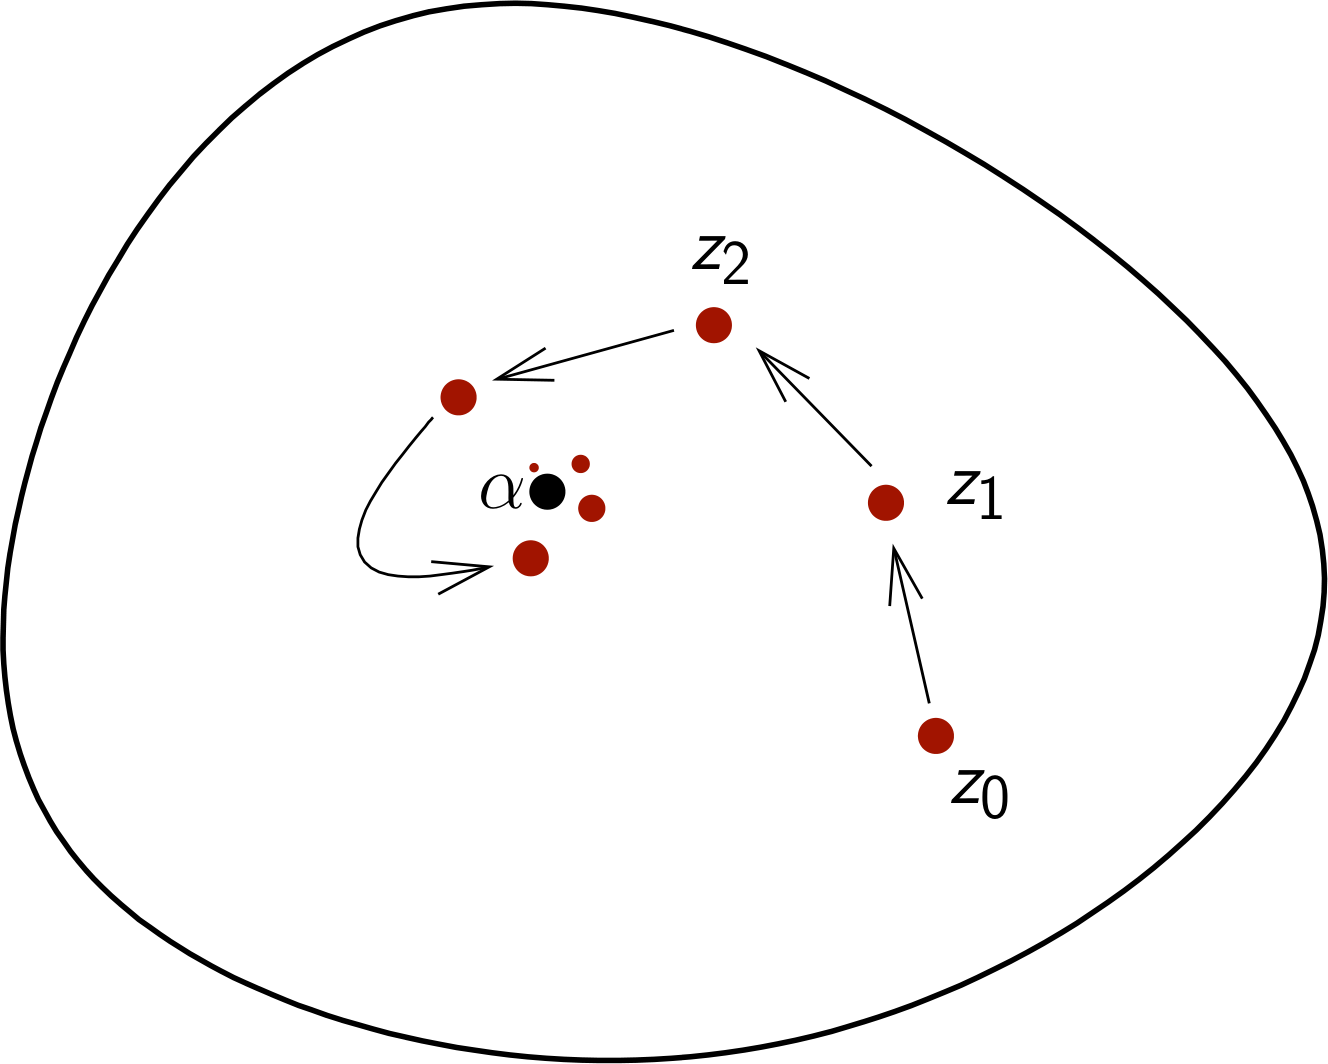
\includegraphics[width=0.5\textwidth]{fig1.png}
    \caption{Every root $\alpha$ of $f$ has a neighborhood of initial conditions
    for which Newton's method works, i.e., the orbit of $z_{0}$ converges to
    $\alpha$.}
    \label{fig:1}
\end{figure}

Ernst Schröder in the year 1870 \cite{9, 10} and, independently, Arthur Cayley
in the year 1879 \cite{2, 3} were the first to propose a global study of
Newton's method. The questions they posed were of the following kind:
\begin{itemize}
    \item If $f$ has several roots, which initial conditions have orbits that
    converge to one or another?
    \item Do all initial conditions lead to convergent orbits? Do these always
    converge to some of the roots of $f$ or are there other possible behaviors?
\end{itemize}

Schröder and Cayley did not get very far in their objectives, but this is how
what we know today as complex dynamics was born, which is the local and global
study of dynamical systems generated by the iteration of analytical functions in
the complex plane.

At this point, it will be useful to define the following concept.

\begin{definition}
Given a root $\alpha$ of the function $f$, we define its \textbf{basin of
attraction} as the set of initial conditions of the plane such that their orbit
under Newton's method converges to $\alpha$, i.e.,
\begin{equation*}
    \mathcal{A}(\alpha)=\{z_{0}\in\mathbb{C} \mid N_{f}^{n}(z_{0})\xrightarrow[n\to\infty]{} \alpha\}.
\end{equation*}
\end{definition}

Both mathematicians solved the problem for the case in which $f$ is a polynomial
of degree 2, proving that each of the two roots of $f$ possesses a half-plane of
initial conditions whose orbits converge to the root in question. These two
basins of attraction are separated by the perpendicular bisector line between
the two roots, formed by initial conditions with orbits that do not converge to
either of the two roots, i.e., initial conditions for which the method ``fails''
(see Figure~\ref{fig:2}).

\begin{figure}[htbp]
    \centering
    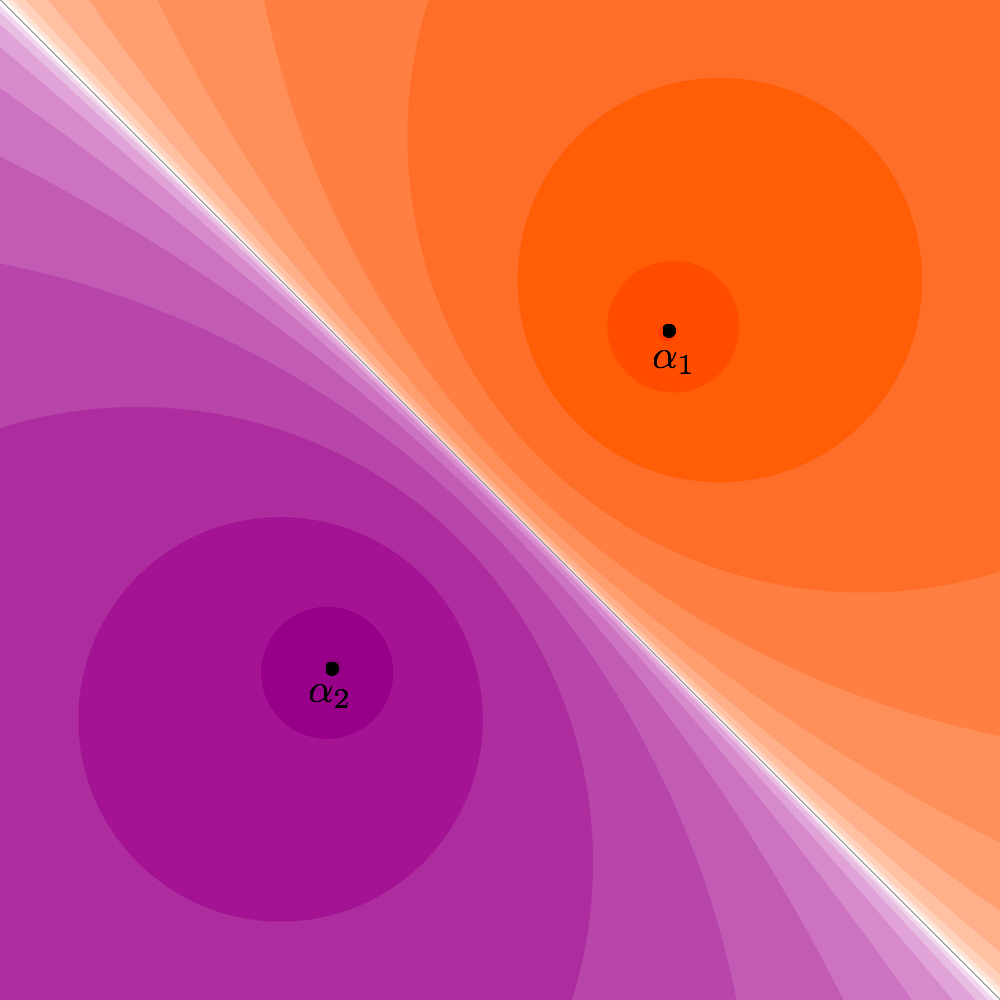
\includegraphics[width=0.5\textwidth]{fig2.png}
    \caption{Newton's method for a polynomial $P$ of degree 2 with roots
    $\alpha_{1}$ and $\alpha_{2}$. In orange, the basin of attraction of
    $\alpha_{1}$ is shown, and in purple that of $\alpha_{2}$. The line that
    separates them is formed by initial conditions for which the method
    ``fails''.}
    \label{fig:2}
\end{figure}

But Cayley gave up regarding degree 3. In his 1880 article \cite{4} he wrote:
\begin{quote}
\dots The division [of the plane into different basins] is done without
difficulty in the quadratic case; but in the next case, that of the cubic
equation, it is not at all obvious what the division is; and the author has not
succeeded in finding it \dots
\end{quote}

The reason Cayley got stuck is that, without knowing it, he was facing a
fractal, without any tool to see it! In Figure~\ref{fig:3}, one can see the
three basins of attraction of Newton's method for a cubic polynomial, each with
a different color. This plane of initial conditions is also called the dynamic
plane or phase plane.

\begin{figure}[htbp]
    \centering
    \begin{subfigure}[b]{0.48\textwidth}
        \centering
        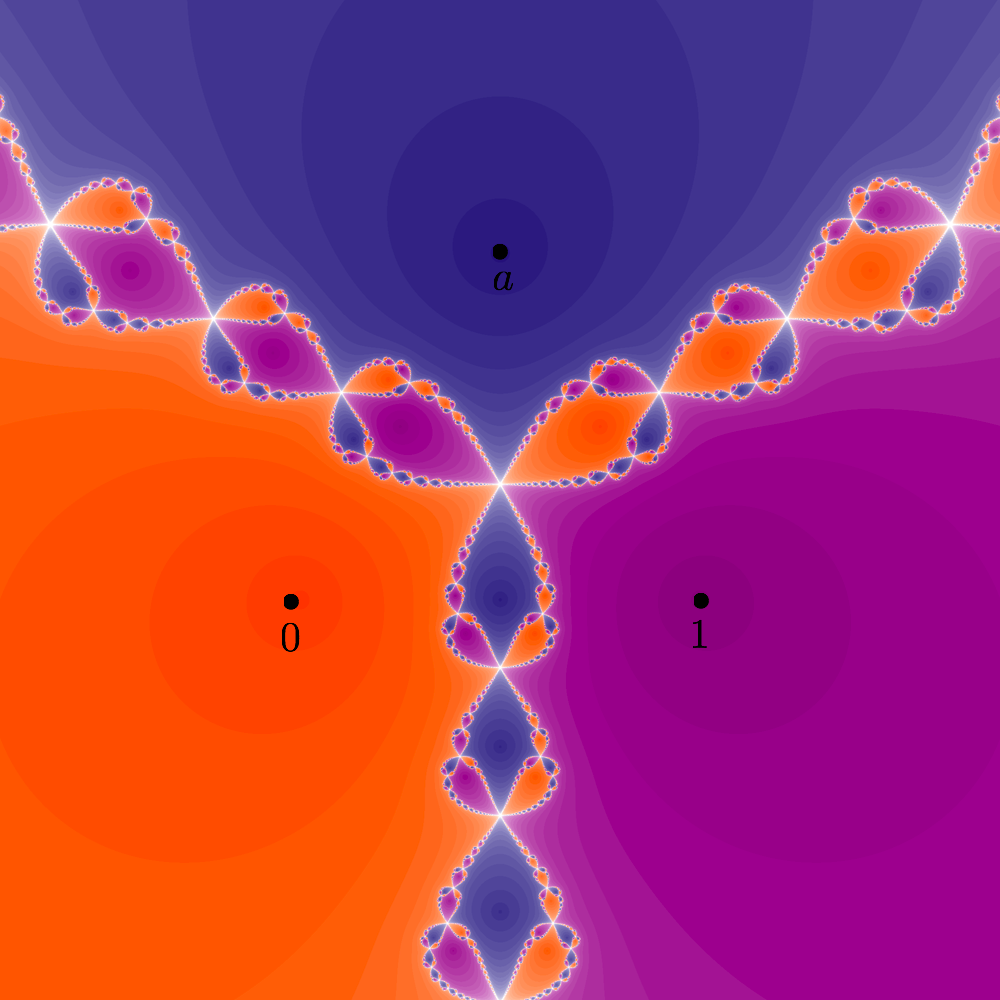
\includegraphics[width=\textwidth]{fig3a.png}
    \end{subfigure}
    \hfill % Adds horizontal space between the two images
    \begin{subfigure}[b]{0.48\textwidth}
        \centering
        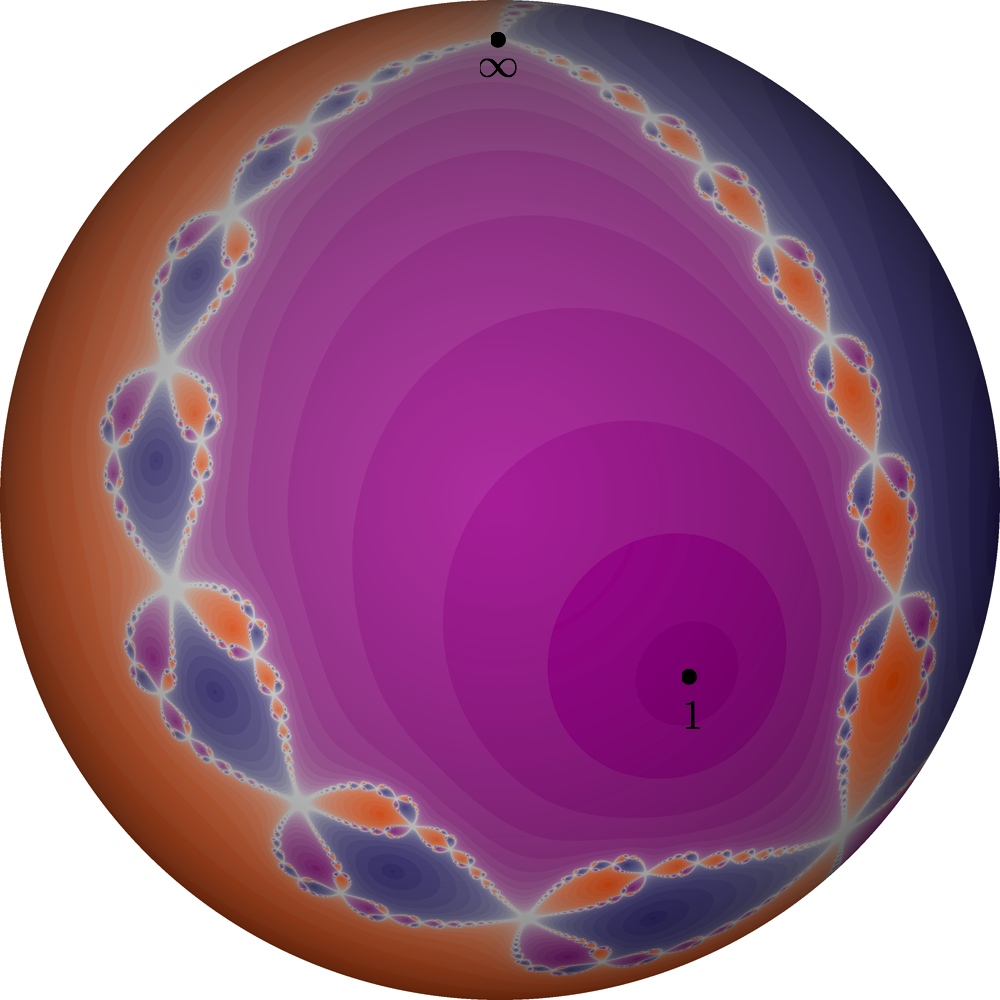
\includegraphics[width=\textwidth]{fig3b.png} 
    \end{subfigure}
    % Main Caption
    \caption{Dynamic space of Newton's method
    $N_{P}(z)=z-\frac{P(z)}{P^{\prime}(z)}$ of the polynomial
    $P(z)=z(z-1)(z-a)$, with $a=0.5+i \sin(\pi/3)$. The initial conditions can
    be seen in the complex plane and also on the Riemann sphere (the
    compactification of $\mathbb{C}$ by adding the point at infinity, which
    corresponds to the north pole). The three basins of attraction of the three
    roots of $P$ are shown in different colors.}
    \label{fig:3}
\end{figure}

It was not until the year 1918 that Pierre Fatou and Gaston Julia undertook a
more systematic study \cite{6, 7, 8} of the iteration of analytical functions,
and established the bases of modern theory, of what we know today as complex
dynamical systems or complex dynamics.

\section{Complex dynamical systems: objectives}

We will set aside Newton's method for the moment, and focus on the iteration of
more general functions which, for simplicity, we will require to be holomorphic
on the Riemann sphere $\hat{\mathbb{C}}=\mathbb{C}\cup\{\infty\}$, or
equivalently, rational functions $F(z)=\frac{P(z)}{Q(z)}$, where $P$ and $Q$ are
polynomials without common roots. Given, then, a rational function
$F:\hat{\mathbb{C}}\rightarrow\hat{\mathbb{C}}$, our goal is to study the
asymptotic behavior of the orbits
\begin{equation*}
    z_{0}, z_{1}=F(z_{0}), \dots, z_{n}=F^{n}(z_{0}), \dots
\end{equation*}
as a function of the initial condition $z_{0}$.

Among the simplest orbits we can find, we highlight the following (see
Figure~\ref{fig:4}):
\begin{itemize}
    \item \textbf{Fixed points:} points $z_{0}$ such that $F(z_{0})=z_{0}$.
    \item \textbf{Periodic points of period $p>1$:} points $z_{0}$ such that
    $F^{p}(z_{0})=z_{0}$ and $F^{k}(z_{0})\neq z_{0}$ for any $k<p$.
    \item \textbf{Preperiodic points:} points $z_{0}$ that are not periodic, but
    such that $F^{k}(z_{0})$ is periodic for some $k>0$.
\end{itemize}

\begin{figure}[htbp]
    \centering
    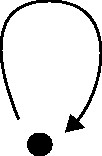
\includegraphics[width=0.08\textwidth]{fig4a.png}\hfill
    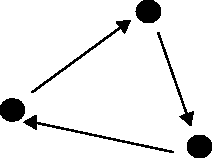
\includegraphics[width=0.15\textwidth]{fig4b.png}\hfill
    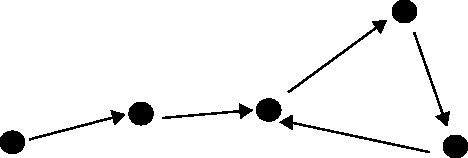
\includegraphics[width=0.34\textwidth]{fig4c.png}
    \caption{From left to right, a fixed point, a periodic orbit of period $p=3$, and a preperiodic orbit.}
    \label{fig:4}
\end{figure}

The mentioned orbits are all finite. An infinite orbit can converge, for
example, to infinity, or to a fixed point, or it may not converge anywhere. With
a slight abuse of language, we will say that the orbit of $z$ converges to a
periodic orbit, say $\{z_{0}, z_{1}, \dots, z_{p-1}\}$, if $F^{np}(z)$ tends to
$z_{i}$ for some $0\le i<p$, as $n\rightarrow\infty$. Note that the exponent is
a multiple of $p$, where $p$ is the length of the periodic orbit.

In studying the phase plane of $F$, the most basic objective is to classify the
initial conditions according to the asymptotic behavior of their orbits. This
can be a very simple problem in some cases and, conversely, in others, it can be
of very difficult solution or, at present, impossible.

\subsection{Invariant sets}

One way to simplify the problem we have just posed is to look for what we call
invariant sets. The definition of these sets is the following.

\begin{definition}
We say that $A \subset \hat{\mathbb{C}}$ is a set:
\begin{itemize}
    \item \textbf{positively invariant}, if $F(A) \subset A$;
    \item \textbf{negatively invariant}, if $F^{-1}(A) \subset A$, where we
    understand that
    \begin{equation*}
        F^{-1}(A)=\{z\in\hat{\mathbb{C}} \mid F(z)\in A\};
    \end{equation*}
    \item \textbf{totally invariant}, if it is both positively and negatively
    invariant, or in other words, if $F^{-1}(A)=A=F(A)$.
\end{itemize}
\end{definition}

Invariant sets are interesting in many areas of mathematics but in particular in
any dynamical system (real or complex, and of any dimension), since they allow
decomposing the system into smaller and perhaps simpler dynamical subsystems to
study. In dynamical systems of $\mathbb{R}^{n}$ we find a multitude of examples
such as invariant manifolds, first integrals, etc., which often allow reducing
the dimension of the system under study.

The smallest invariant sets are the orbits themselves. Indeed, what we call the
positive orbit of $z_{0}$ and denote by
\begin{equation*}
    \mathcal{O}^{+}(z_{0})=\{z_{0}, z_{1}, \dots, z_{n}=F^{n}(z_{0}), \dots\}
\end{equation*}
is positively invariant. The grand orbit of $z_{0}$
\begin{equation*}
    \mathcal{O}(z_{0})=\{z\in\hat{\mathbb{C}} \mid F^{p}(z)=F^{q}(z_{0}) \text{ for some } p,q\in\mathbb{N}\}
\end{equation*}
is totally invariant (see Figure~\ref{fig:5}).

\begin{figure}[htbp]
    \centering
    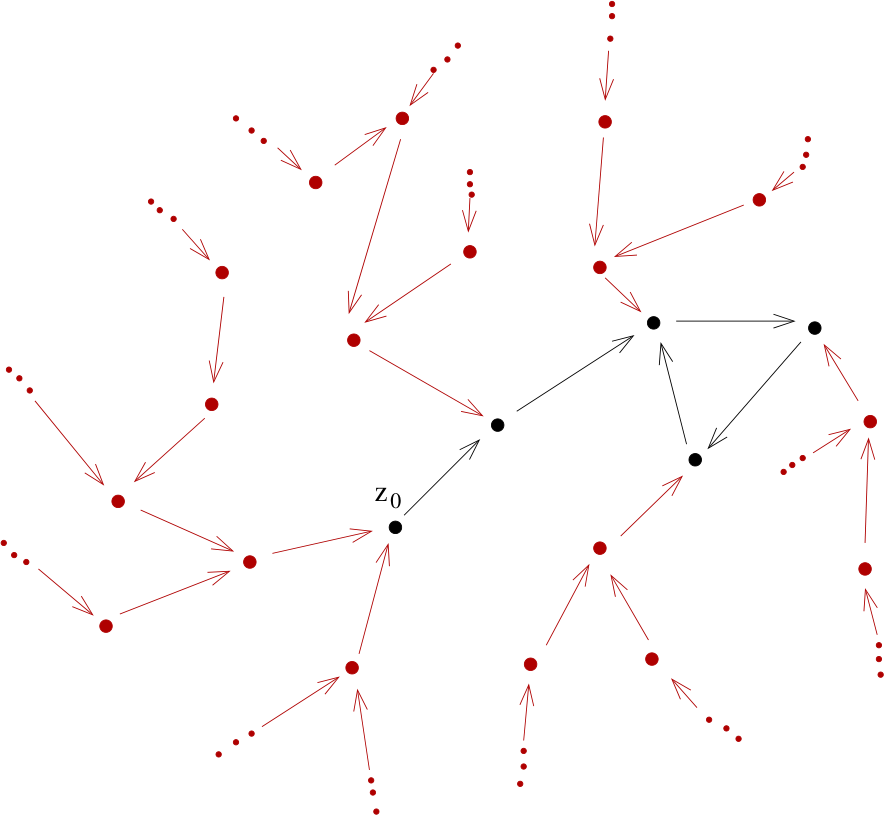
\includegraphics[width=0.5\textwidth]{fig5.png}
    \caption{The grand orbit of a point $z_{0}$, $\mathcal{O}(z_{0})$, consists
    of the set of points ``related'' to $z_{0}$ through iterates of $F$. In black
    we see the positive orbit of $z_{0}$, which in this case is finite. We observe
    that if $z$ belongs to $\mathcal{O}(z_{0})$, then
    $\mathcal{O}(z)=\mathcal{O}(z_{0})$.}
    \label{fig:5}
\end{figure}

Let us return now to examine the dynamical system generated by Newton's method,
and consider what invariant sets we can observe in it.

Recall that if $\alpha$ is a root of a polynomial $P$, the local study of
Newton's method told us that $\alpha$ is equipped with a neighborhood $U$ of
initial conditions whose orbits converge to $\alpha$. In the previous
terminology, this is saying that $U$ belongs to the basin of attraction of
$\alpha$ and, in fact, this basin consists of all preimages (of all orders) of
$U$. That is:
\begin{equation*}
    \mathcal{A}(\alpha)=\{z_{0}\in\mathbb{C} \mid N_{P}^{n}(z_{0})\xrightarrow[n\to\infty]{} \alpha\}=\bigcup_{n\ge 1} N_{P}^{-n}(U).
\end{equation*}

Observe that $U$ is a positively invariant set, while the entire basin
$\mathcal{A}(\alpha)$ is totally invariant. In general, a basin of attraction
$\mathcal{A}(\alpha)$ is a set that is:
\begin{itemize}
    \item open, by continuity;
    \item totally invariant, by definition, since it is formed by grand orbits,
    and these are totally invariant;
    \item possibly formed by infinitely many connected components. It has a main
    one $\mathcal{A}^{*}(\alpha)$ which is the one containing $\alpha$.
\end{itemize}

In Figure~\ref{fig:6}, we can see the dynamic plane of Newton's method for
another cubic polynomial. We observe three basins of attraction in three
different colors. Apparently (and in fact, it is so) one of these is formed by a
single connected component, while the others have infinitely many.

\begin{figure}[htbp]
    \centering
    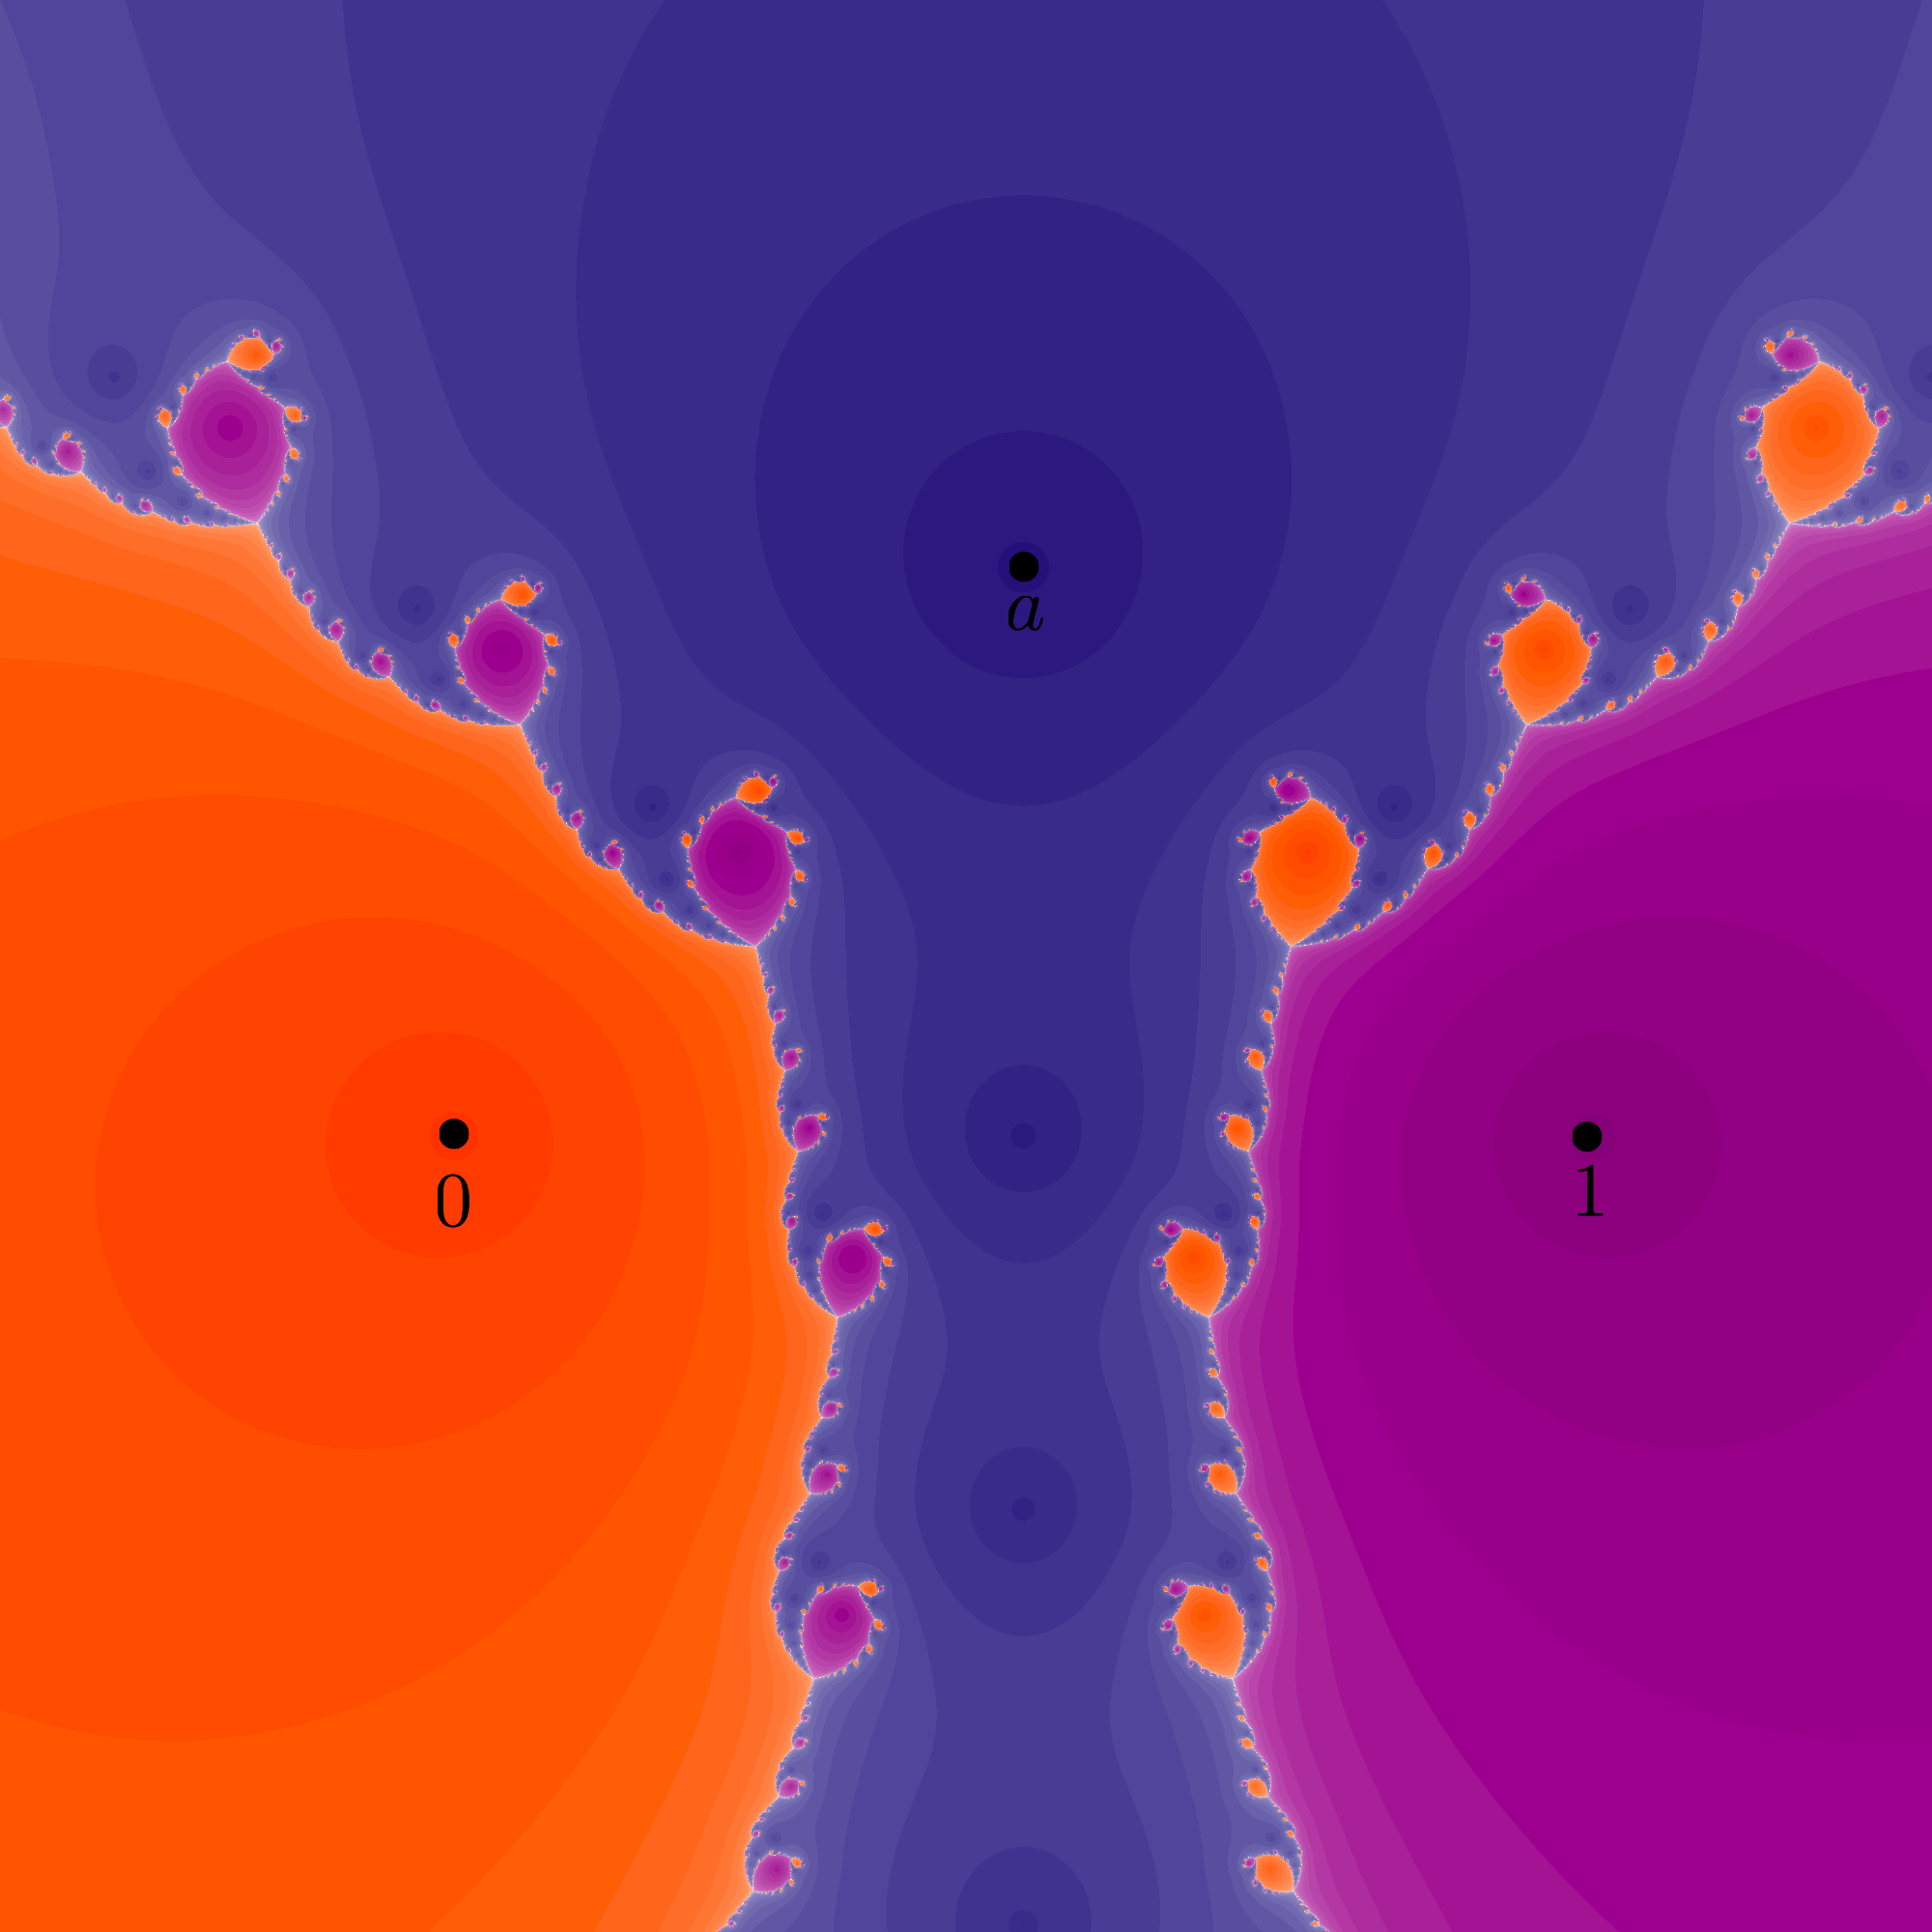
\includegraphics[width=0.5\textwidth]{fig6.png}
    \caption{Phase plane of Newton's method $N_{P}$ for $P(z)=z(z-1)(z-a)$ with
    $a=\frac{1}{2}(1+i)$. We see three totally invariant basins of attraction. One
    of these, that of $a$, is formed by a single connected component, while the
    other two have infinitely many.}
    \label{fig:6}
\end{figure}

Observe at this point that, although we defined the concept of basin of
attraction for Newton's method, this is easily generalizable to other functions.
Given a rational function $F$ with a fixed (or periodic) point that attracts the
orbits of a neighborhood (points with this property are called attractors), its
basin of attraction is, analogously, the set of orbits that converge to it. Thus
defined, any basin of attraction has all the mentioned properties: it is open,
totally invariant, and possibly formed by infinitely many connected components.

It is not difficult to check that if a set $A$ is totally invariant, its
complement and its boundary must also be totally invariant. Therefore, we obtain
the second example of invariant sets: if $\mathcal{A}(\alpha)$ is a basin of
attraction, its boundary is also totally invariant. By definition, this set is
closed and cannot have an interior.

\section{The basic partition: the Julia and Fatou sets}

There is a fundamental difference between the two examples of totally invariant
sets we have presented: the basins of attraction belong to what we call the
Fatou set or stable set, while their boundaries belong to the Julia set or
chaotic set. Let us see now how these two sets are defined, which are in more
than one aspect complementary to each other. We previously need the concept of
normality of the family of iterates in a certain open set of the plane.

\begin{definition}
Let $F:\hat{\mathbb{C}}\rightarrow\hat{\mathbb{C}}$. We say that the family of
iterates $\{F^{n}\}_{n\in\mathbb{N}}$ is \textbf{normal} in an open set
$U\subset\hat{\mathbb{C}}$ if every subsequence of $\{F^{n}\}_{n\in\mathbb{N}}$
has a sub-subsequence that converges uniformly on compact subsets of $U$
(possibly to $\infty$).
\end{definition}

Informally, the family of iterates is normal in an open set when all points of
the open set behave similarly under the iteration of $F, $ which is why we
relate this concept to stability.

\begin{definition}
The \textbf{Fatou set}, $\mathcal{F}(F)$, is defined as the set of points
$z\in\hat{\mathbb{C}}$ for which the family of iterates
$\{F^{n}\}_{n\in\mathbb{N}}$ is normal in some neighborhood $U$ of $z$. Its
complement is called the \textbf{Julia set}. That is,
$\mathcal{J}(F)=\hat{\mathbb{C}}\backslash\mathcal{F}(F)$ is the set of points
for which the family of iterates is not normal in any of its neighborhoods.
\end{definition}

From the definition itself, it is not difficult to deduce that any basin of
attraction of a fixed point $\alpha$ belongs to the Fatou set, since the
sequence of iterates of $F$ itself converges uniformly on compact sets to the
constant function $G(z)\equiv\alpha$. The boundary of
$\mathcal{A}=\mathcal{A}(\alpha)$, on the other hand, belongs to the Julia set.
Let us give a short proof of this.

\begin{proof}
Indeed, if $z_{0}$ belongs to $\partial\mathcal{A}$, any neighborhood $U$ of
$z_{0}$ contains points of $\mathcal{A}$ and of its complement. Any limit
function $G$ of some subsequence of iterates would have to be equal to $\alpha$
for all $z \in U \cap \mathcal{A}$, which is a non-empty open set. Since $G$ is
analytic (by Weierstrass's theorem), the identity theorem (or analytic
continuation principle) would tell us that $G$ must be identically equal to
$\alpha$ on the whole of $U$, which contradicts the fact that no subsequence of
iterates of $z_{0}$ can converge to $\alpha$, because $z_{0}$ does not belong to
the basin of attraction.
\end{proof}

From the definition itself, we can see that the Julia and Fatou sets are totally
invariant, since the concept of normality is an asymptotic concept associated
with grand orbits. We will see next that these two sets are completely opposite,
both topologically and dynamically. For this reason, we say that they form the
basic partition of the phase space. Figure~\ref{fig:7} shows phase planes of
different functions where we can see examples of Fatou and Julia sets.

\begin{figure}[htbp]
    \centering
    % Top Row
    \begin{subfigure}[b]{0.48\textwidth}
        \centering
        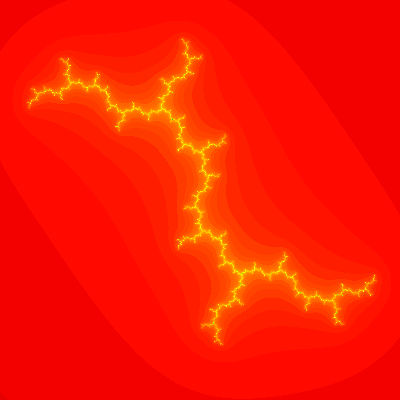
\includegraphics[width=\textwidth]{fig7a.png}
        \caption{$F(z) = z^2 + i$.}
        \label{fig:7a}
    \end{subfigure}
    %\hfill % Adds horizontal space between the two images
    \begin{subfigure}[b]{0.48\textwidth}
        \centering
        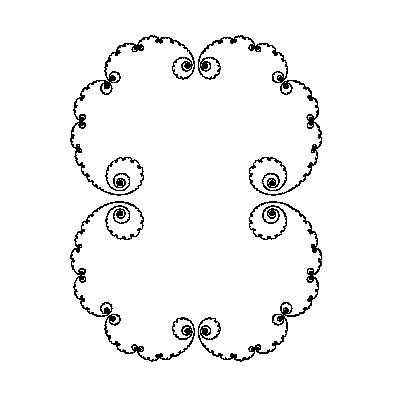
\includegraphics[width=\textwidth]{fig7b.png} 
        \caption{$F(z) = z^2 + 0.25$.}
        \label{fig:7b}
    \end{subfigure}

    %\vspace{0.5cm} % Adds vertical space between the rows

    % Bottom Row
    \begin{subfigure}[b]{0.48\textwidth}
        \centering
        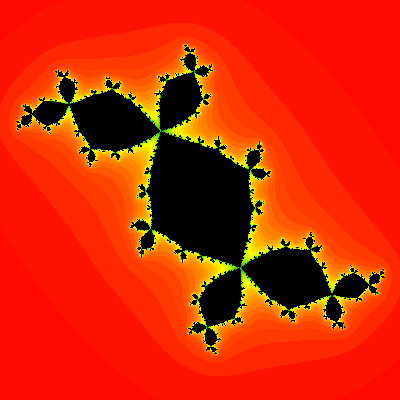
\includegraphics[width=\textwidth]{fig7c.png}
        \caption{$F(z) = z^2 - 0.122\ldots + 0.744\ldots i$.}
        \label{fig:7c}
    \end{subfigure}
    %\hfill
    \begin{subfigure}[b]{0.48\textwidth}
        \centering
        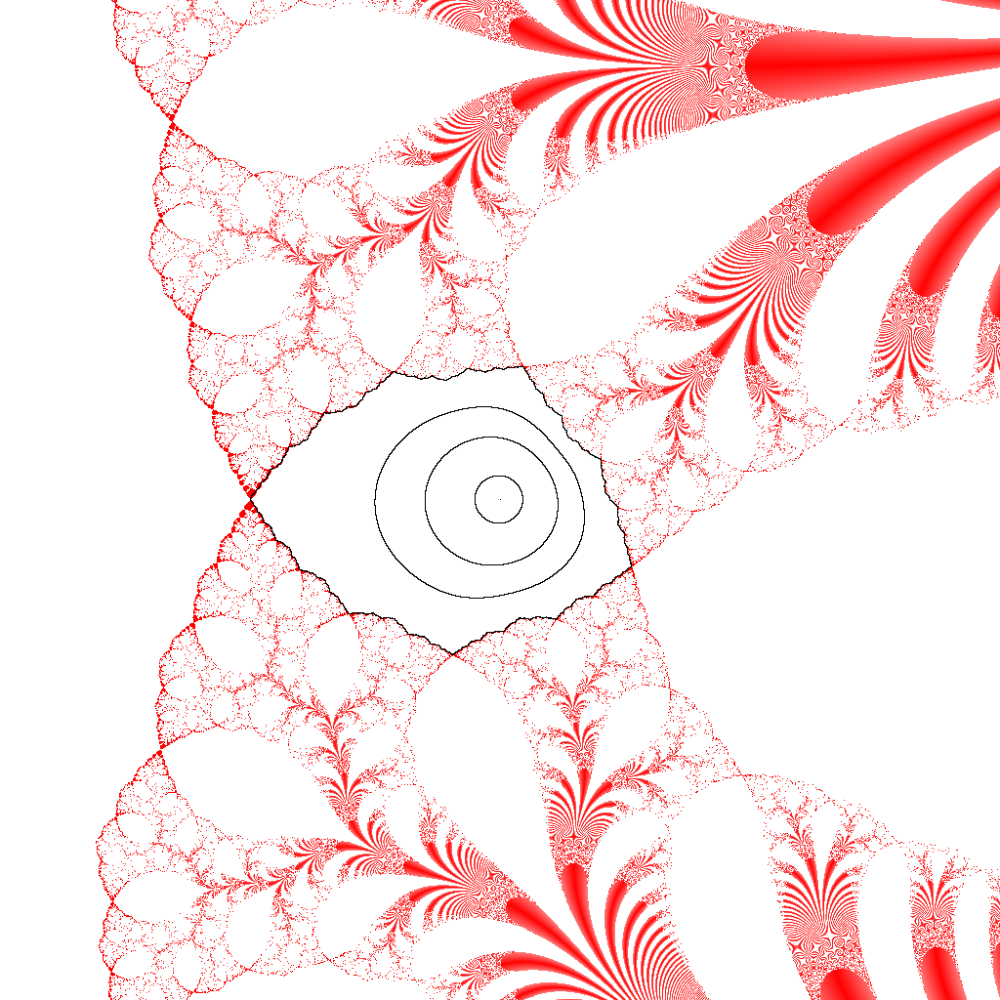
\includegraphics[width=\textwidth]{fig7d.png}
        \caption{$F(z) = e^{2\pi i \theta}ze^z$, $\zeta = \frac{1 - \sqrt{5}}{2}$.}
        \label{fig:7d}
    \end{subfigure}

    % Main Caption
    \caption{a) In red we see the basin of attraction of infinity which
    coincides with $\mathcal{F}(F)$. The Julia set (yellow) is a dendrite
    (closed, connected, and with no interior). b) In white we see
    $\mathcal{F}(F)=\mathcal{A}(\infty)$. The Julia set (black) is a Cantor set.
    c) In red we see $\mathcal{A}(\infty)$ and in black its complement $K$,
    known as ``Douady's rabbit''. The common boundary to these two sets is
    $\mathcal{J}(F)$. The points in the interior of $K$ form part of the basin
    of attraction of a periodic orbit of period 3. d) In red we see
    $\mathcal{J}(F)$, which consists of a set of ``filaments''. In white we see
    $\mathcal{F}(F)$ and in black some of its orbits, all accumulating on
    invariant curves, where $F$ is basically a rotation of irrational angle.}
    \label{fig:7}
\end{figure}

\subsection{Topological properties of the Julia set}

Next, we will state several topological properties of the Julia set of a
rational function. Some are simple to prove, while others require proofs beyond
the scope of this text.

\begin{proposition}
Let $F:\hat{\mathbb{C}}\rightarrow\hat{\mathbb{C}}$ be a holomorphic function
and let $\mathcal{J}$ be its Julia set. Then:
\begin{itemize}
    \item $\mathcal{J}$ is closed and non-empty.
    \item $\text{int}(\mathcal{J})=\emptyset$ or else
    $\mathcal{J}=\hat{\mathbb{C}}$.
    \item $\mathcal{J}$ is ``self-similar'', that is, in all its parts we find
    scaled copies of the original set.
\end{itemize}
\end{proposition}

There are examples of topologically very different Julia sets, as we have begun
to see in Figure~\ref{fig:7}. As a small sample, we mention that there exist
examples of different Julia sets that are:
\begin{itemize}
    \item connected, disconnected, or Cantor sets;
    \item locally connected and non-locally connected;
    \item with Lebesgue measure zero and with positive measure (but without
    interior!);
    \item with Hausdorff dimension $1+t$ for all $t\in(0,1]$.
\end{itemize}

It is worth noting that the existence of rational functions with Julia sets of
positive measure, but without interior, was a highly disputed conjecture for
more than twenty years, which was resolved positively very recently by X. Buff
and A. Chéritat (2005). These authors showed that even within the simplest
families (quadratic polynomials) one can find Julia sets with this property.

\subsection{Dynamical properties of the Julia sets}

We could almost say that, in a natural way, the dynamics on the Julia set is
unstable, since it is the boundary between different stable behaviors and,
therefore, must reflect the tension between them. In fact, the orbits of the
Julia set exhibit all the properties usually associated with the concept of
chaos. Without defining what it means for a function to be chaotic (which is
actually just a matter of convention), we will list some of these
characteristics, without proof. The dynamics of the orbits of the Julia set thus
exhibit the following properties:
\begin{enumerate}
    \item $F|_{\mathcal{J}}$ is sensitive with respect to initial conditions.
    Intuitively, this means that orbits that start very close to each other
    eventually diverge. Formalizing, there exists $k>0$ such that for every
    $z_{0}\in\mathcal{J}$ and for every $\epsilon>0$, there exists
    $z_{1}\in\mathcal{J}$ with $|z_{0}-z_{1}|<\epsilon$ and there exists $n>0$
    such that $|F^{n}(z_{0})-F^{n}(z_{1})|\ge k$.
    \item The (grand) orbits are dense in the whole of $\mathcal{J}$. For any
    point $z\in\mathcal{J}$, the grand orbit of $z$ is dense in $\mathcal{J}$.
    In fact, the backward orbit $\mathcal{O}^{-}(z)$ (i.e., the set of preimages
    of $z$) is also dense in $\mathcal{J}$.
    \item $F$ is transitive on $\mathcal{J}$. Informally, this means that $F$
    ``mixes'' all orbits. Formally, for any neighborhoods $U, V$ of points in
    $\mathcal{J}$, we have $F^{n}(U)\cap V\neq\emptyset$ for some $n$.
    \item The (non-attracting) periodic points of $F$ are dense in
    $\mathcal{J}$. In other words, we find periodic points as close as we want
    to any point of $\mathcal{J}$. Note that they cannot be attracting, since
    these form part of the stable set.
\end{enumerate}

Note that from the previous properties, for example from the second or the
third, the following fact is deduced.

\begin{proposition}
$\mathcal{J}$ cannot have any proper totally invariant subset. That is, there
does not exist any non-empty, totally invariant subset $A\subset\mathcal{J}$
such that $\overline{A}\neq\mathcal{J}$.
\end{proposition}

In other words, we can say that the Julia set can no longer be decomposed
further in the dynamical sense, that is, into significant totally invariant
parts. This is not the case for its complement, as we will see next.

\section{The Fatou or stable set}

Recall that the Fatou set $\mathcal{F}$, the complement of $\mathcal{J}$, is
open and contains all initial conditions with orbits showing stable asymptotic
behavior. In fact, we have already seen an example: the basin of attraction of
an attracting fixed point is always part of $\mathcal{F}$. The condition for a
fixed point to be attracting is that $|F^{\prime}(z_{0})|<1$, which can be
easily checked by looking at the first terms of the Taylor expansion of $F$ near
$z_{0}$.

It is natural to ask, however, what other behaviors are possible for the orbits
in $\mathcal{F}$. Below we see some examples.

\paragraph{Example 1. Periodic basin of attraction.}
The orbits ``converge'' to an attracting periodic orbit, in the sense defined
above. Generalizing the case of a fixed point, given a periodic orbit $\{z_{0},
z_{1}, \dots, z_{p-1}\}$ of period $p$, the necessary and sufficient condition
for it to be attracting is that its multiplier has modulus less than 1, i.e.:
\begin{equation*}
    |\lambda|=|(F^{p})^{\prime}(z_{i})|=|F^{\prime}(z_{0})F^{\prime}(z_{1})\cdots F^{\prime}(z_{p-1})|<1.
\end{equation*}

In Figure~\ref{fig:8} we see the phase plane of the function $F(z)=z^{2}-1$.

\begin{figure}[htbp]
    \centering
    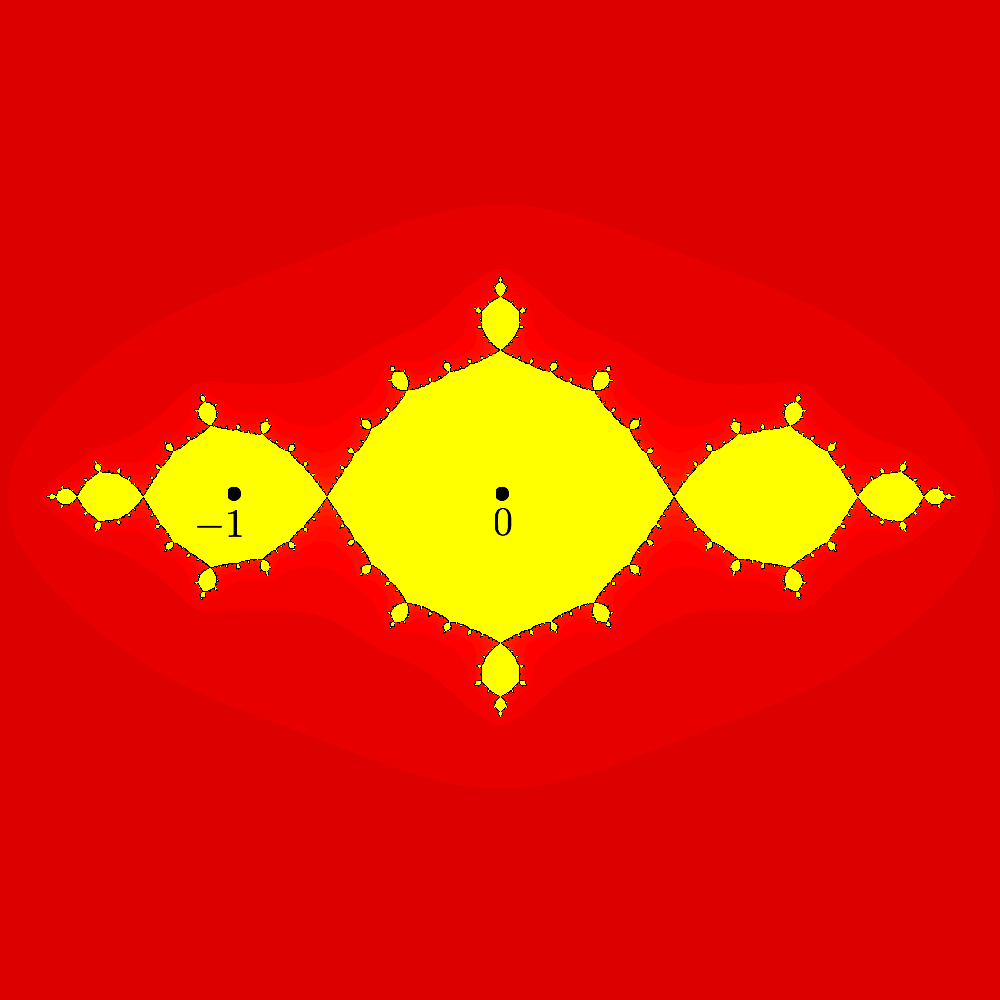
\includegraphics[width=0.5\textwidth]{fig8.png}
    \caption{The phase plane of $F(z)=z^{2}-1$. The orbit $\{0, -1\}$ is
    2-periodic and attracting. In yellow we see its basin of attraction, part of
    the Fatou set. In red we see the basin of attraction of the point at infinity.
    The common boundary of both basins is the Julia set.}
    \label{fig:8}
\end{figure}

The orbit $\{0, -1\}$ is an attracting period-2 orbit. This is surrounded by an
immediate basin of attraction that corresponds to the two yellow (open)
components containing it. The union of all preimages of these forms the totality
of the basin drawn in yellow. Its complement, drawn in shades of red, is another
basin of attraction, in this case of the point at infinity. The common boundary
between the two basins, both of the stable set, is precisely the Julia set (in
black).

\paragraph{Example 2. Parabolic basin.}
Another example of stable behavior is found by considering what we call
parabolic (attraction) basins. They are very similar to the previous ones, but
with the difference that the ``limit'' points (fixed or periodic) are on the
boundary of the basin, and not in its interior. As before, we also have a
necessary and sufficient condition for a periodic orbit $\{z_{0}, z_{1}, \dots,
z_{p-1}\}$ of period $p$ to be parabolic, and this is that its multiplier has
modulus exactly 1, with the property
\begin{equation*}
    |\lambda|=|(F^{p})^{\prime}(z_{0})|=e^{2\pi i p/q}, \quad p,q\in\mathbb{Z}, \quad \gcd(p,q)=1.
\end{equation*}

In Figure~\ref{fig:9} we can see the phase plane of the polynomial
$F(z)=z^{2}+0.25$, which has a fixed point at $z_{0}=1/2$, with multiplier
$\lambda=1$.

\begin{figure}[htbp]
    \centering
    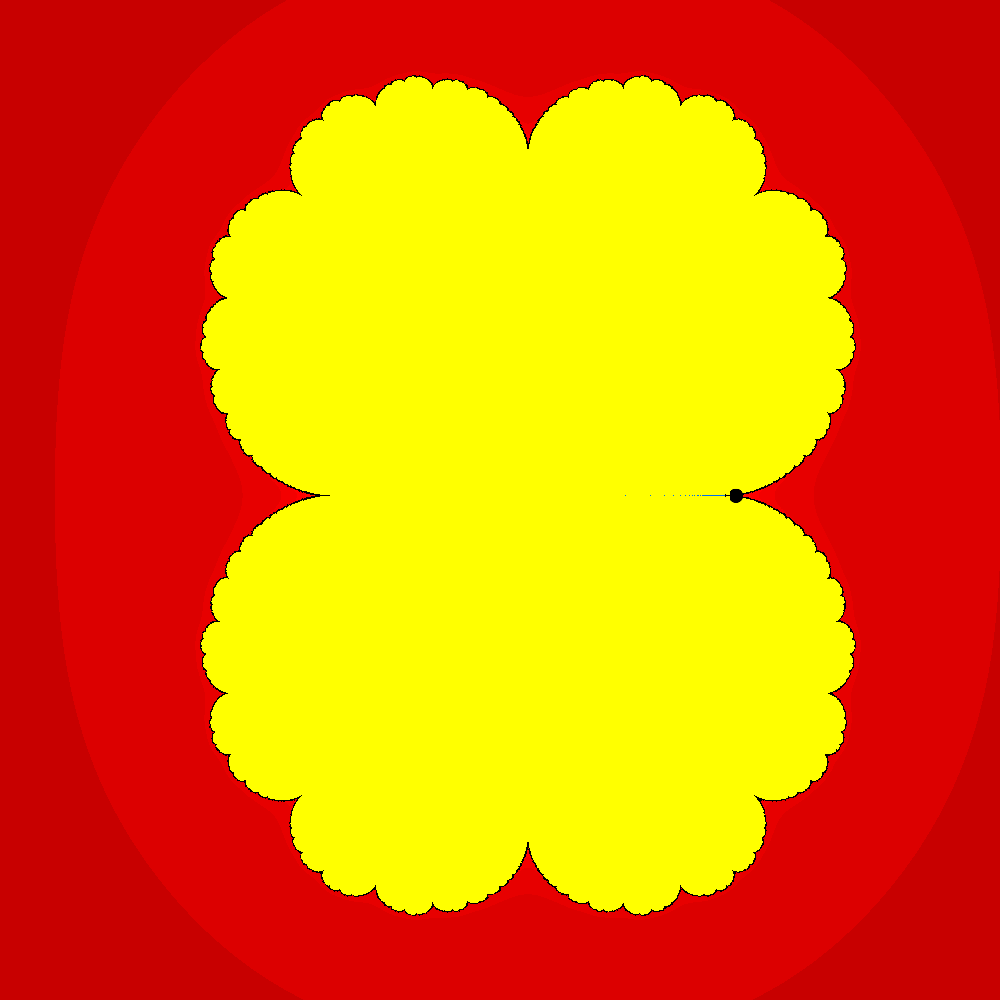
\includegraphics[width=0.5\textwidth]{fig9.png}
    \caption{Phase plane of $F(z)=z^{2}+0.25$, for which $z_{0}=1/2$ is a
    parabolic fixed point. In yellow, its parabolic basin is shown, which has
    $z_{0}$ on its boundary (right). In red, the basin of attraction of infinity.}
    \label{fig:9}
\end{figure}

In the figure, we see in yellow its parabolic basin of attraction, in this case
formed by a single connected component. All points of this color have orbits
that converge to $z_{0}$, located on the boundary. As before, in red we see the
basin of attraction of infinity and, in black, the common boundary that
corresponds to the Julia set (in this case a Jordan curve, not differentiable at
any of its points).

\paragraph{Example 3. Rotation disk.}
A very different example of a stable component is what is called a rotation
disk, also known as a Siegel disk in honor of Carl Siegel (1896--1981), who gave
sufficient conditions for its existence.

What is known as a fixed rotation disk for $F$ is an open set $U$ conformally
equivalent to the unit disk, which contains a fixed point $z_{0}$ in its
interior, and such that $F|_{U}$ is conformally conjugate to a rigid rotation
$\mathcal{R}_{\theta}(z)=e^{2\pi i\theta}z$ on the unit disk, where
$\theta\in\mathbb{R}\backslash\mathbb{Q}$. This means that there exists a
conformal homeomorphism $h:U\rightarrow\mathbb{D}$ such that $h\circ F =
\mathcal{R}_{\theta}\circ h$.

This means that the orbits inside $U$ lie on invariant curves and, on these,
they behave like an irrational rotation, i.e., they accumulate densely over the
entire curve.

In Figure~\ref{fig:10} we show the phase plane of the function $F(z)=\lambda
z(1-z)$ where $\lambda=e^{2\pi i \frac{1-\sqrt{5}}{2}}$.

\begin{figure}[htbp]
    \centering
    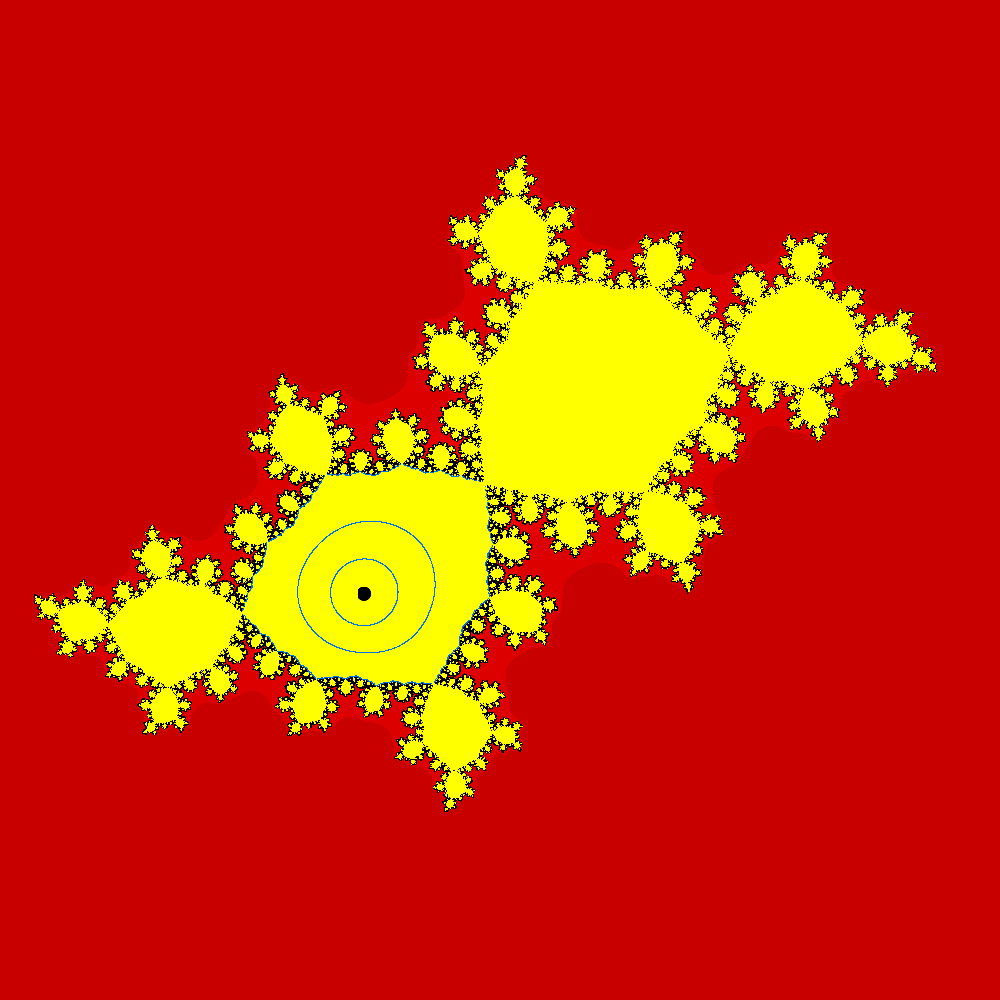
\includegraphics[width=0.5\textwidth]{fig10.png}
    \caption{Phase plane of $F(z)=\lambda z(1-z)$ where $\lambda=e^{2\pi i
    \frac{1-\sqrt{5}}{2}}$. In yellow a fixed Siegel disk around $z=0$ and all its
    preimages are shown. In red, the basin of attraction of infinity.}
    \label{fig:10}
\end{figure}

The black point corresponds to a fixed point and the curves around it are some
of the invariant curves. The orbit of any of its points is dense on the curve.
The yellow component containing these elements is the fixed Siegel disk $U$. All
other components of the same color are preimages of $U$ and together they form
the grand orbit of $U$, which is totally invariant. In red we see again the
basin of attraction of infinity and in black the common boundary which is the
Julia set. In this case, we also have sufficient conditions that ensure the
existence of this type of stable components. Siegel already proved that if
$z_{0}$ is a fixed point with multiplier $\lambda=F^{\prime}(z_{0})=e^{2\pi
i\theta}$, with $\theta$ a Diophantine irrational number, then there is always a
Siegel disk around $z_{0}$. More recently (1971), this condition was improved by
Brjuno \cite{1}, by proving the same fact for all numbers $\theta$ in the Brjuno
set, a set of irrationals that includes Diophantine numbers. Finding necessary
conditions for the existence of rotation disks is a more difficult problem that
depends on the specific family being studied. In fact, in most cases, this is
still an open problem.

\paragraph{Example 4. Rotation ring.}
This is an example very similar to the previous one, with the only difference
that the domain is conformally equivalent to an annulus, instead of a disk. In
this annulus, we have the same phenomenon as before, i.e., the function is
conjugate to an irrational rotation and, therefore, all orbits are dense on
invariant curves. These rings are also known as Herman rings in honor of Michel
Herman (1942--2000), who found the first examples.

Rotation rings differ from the previous examples in that they are not associated
with any periodic orbit. Because of this, we do not have any simple criterion
from which their existence can be deduced for a specific function.

As a consequence of the maximum modulus principle, it is established that any
rotation ring requires the presence of a pole of the function. For this reason,
we can never find rotation rings in the phase planes of polynomials or entire
functions in general.

In Figure~\ref{fig:11} we can see the phase plane of the rational function
$F(z)=z^{2}\frac{z-a}{1-\bar{a}z}$, for a certain conveniently chosen value of
$a$. In gray, a Herman ring is shown, inside of which one of its invariant
curves is drawn. All white ring-shaped components are preimages (of different
orders) of the main ring. The disk-like white components form part of the basin
of infinity and the basin of zero, which in this case are both, zero and
infinity, attracting fixed points.

\begin{figure}[htbp]
    \centering
    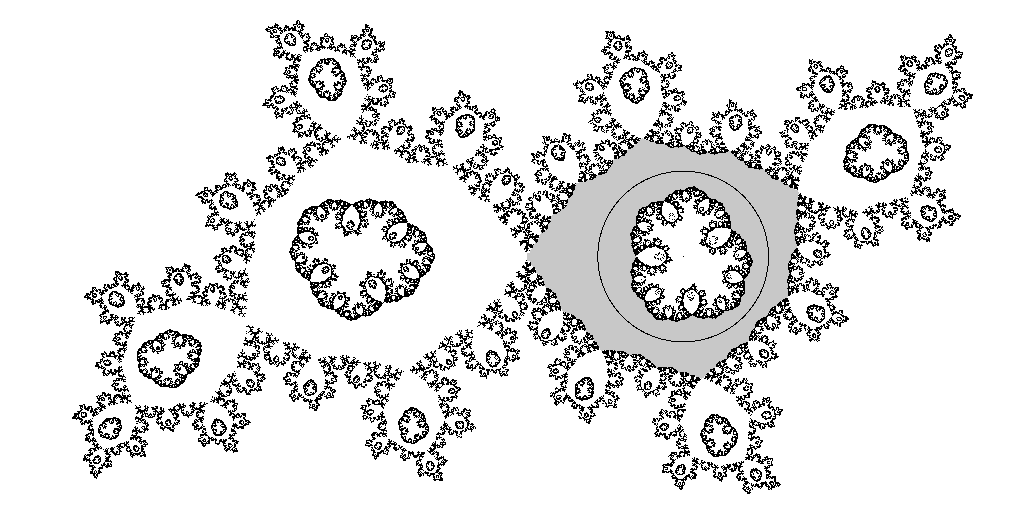
\includegraphics[width=0.65\textwidth]{fig11.png}
    \caption{Phase plane of $F(z)=z^{2}\frac{z-a}{1-\bar{a}z}$ for a certain
    conveniently chosen value of $a$. In gray, a Herman ring is shown, inside of
    which one of its invariant curves is drawn.}
    \label{fig:11}
\end{figure}

\paragraph{Example 5. Parabolic domain at infinity.}
A fixed parabolic domain at infinity is an open set $U$ of the plane such that
all its orbits converge toward the point at infinity, which must be an essential
singularity. These components are also known by the name of Baker domains in
honor of Noel Baker (1932--2001), who made the first exhaustive studies of them.

By definition, then, these stable components only exist in transcendental
functions (i.e., with essential singularities). We find ourselves again with a
type of components that is not associated with any periodic orbit either.

In Figure~\ref{fig:12} we see the phase plane of $F(z)=z+a+b\sin(z)$ with $a$
and $b$ chosen appropriately so that the Fatou set has a Baker domain, shown in
red. The orbits inside this set escape to the right, tending toward infinity,
with an essentially linear velocity. In blue, the preimages of the Baker domain
can be seen.

\begin{figure}[htbp]
    \centering
    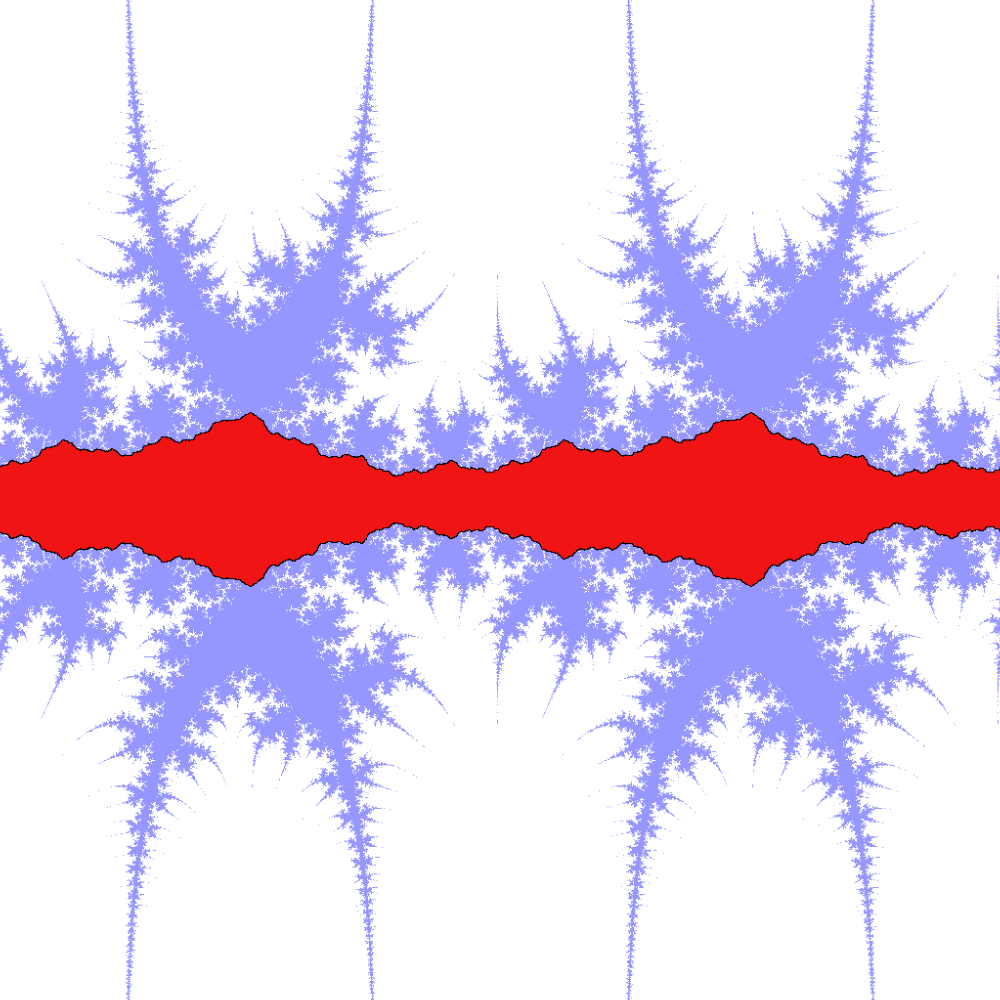
\includegraphics[width=0.5\textwidth]{fig12.png}
    \caption{Phase plane of $F(z)=z+a+b\sin(z)$ with $a$ and $b$ chosen appropriately so that the Fatou set has a Baker domain, shown in red. Orbits inside this domain tend toward infinity with linear velocity. In blue we see all preimages of the Baker domain.}
    \label{fig:12}
\end{figure}

\paragraph{Example 6. Wandering domains.}
A wandering domain is an open set $U$ such that $F^{n}(U)\cap
F^{m}(U)=\emptyset$ for all $n, m \in \mathbb{N}$ with $n \neq m$. That is,
wandering domains are neither periodic nor preperiodic components.

In Figure~\ref{fig:13} we see the dynamic plane of the transcendental function
$F(z)=z+2\pi+\sin(z)$. The central components colored gray, centered at the
points $z_{k}=(2k+1)\pi$, correspond to an orbit of wandering domains. The
smaller ones are preimages of these.

\begin{figure}[htbp]
    \centering
    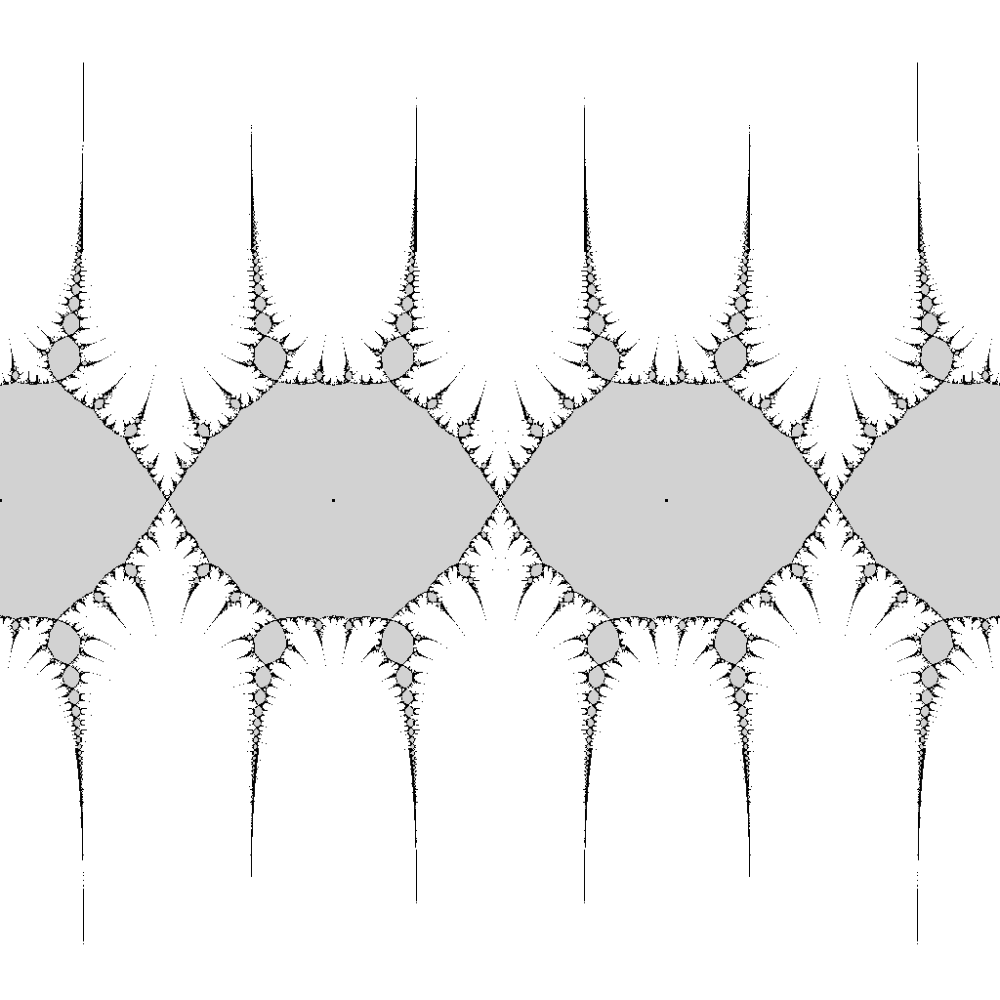
\includegraphics[width=0.5\textwidth]{fig13.png}
    \caption{Phase plane of the transcendental function $F(z)=z+2\pi+\sin(z)$. The central components colored gray correspond to an orbit of wandering domains.}
    \label{fig:13}
\end{figure}

Fatou and Julia proved that, in theory, these domains were possible. It was not
until much later, in 1985, that Dennis Sullivan proved the celebrated theorem
establishing that rational functions cannot have wandering domains. This result
opened a new era of complex dynamics, not because of the statement itself, but
because of the techniques used in its proof, which were highly innovative at
that time.

\begin{theorem}[Sullivan, \cite{11}]
Rational functions ($F(z)=\frac{Q_{1}(z)}{Q_{2}(z)}$, where $Q_{1}, Q_{2}$ are
polynomials) do not have wandering domains.
\end{theorem}

\subsection{Classification of stable components}

The previous examples have shown us a variety of components of the Fatou set,
where each exhibits a different behavior of the iterates of the function. Fatou,
in 1918, did not have the possibility to ``see'' these examples, but
nevertheless, he was able to prove the following classification theorem.

\begin{theorem}[Fatou, 1918]
Let $U$ be a periodic connected component of $\mathcal{F}(F)$ where $F$ is a
rational function on $\hat{\mathbb{C}}$. Then $U$ is part of a basin of
attraction, of a parabolic basin, of a rotation disk, or of a rotation ring.
\end{theorem}

If $F$ is transcendental, $U$ can also be a parabolic domain at infinity. If $U$
is not periodic, then $U$ is a preimage of some of the previous ones or it can
be a wandering domain.

Fatou found examples of most of these behaviors, and conjectured that probably
rotation domains did not exist. It was not until many years later that their
existence could be proven, as we have mentioned before, as well as the
non-existence of wandering domains for rational functions.

\subsection{Newton's method revisited}

We had seen that, given a polynomial $P(z)$ with roots $\alpha_{1}, \dots,
\alpha_{k}$, each is equipped with its basin of attraction under Newton's method
$F(z)=N_{P}(z)$, consisting of all initial conditions with orbits that converge
toward the root in question. In fact, it is simple to check that
$N_{P}(\alpha_{i})=\alpha_{i}$ and that $N_{P}^{\prime}(\alpha_{i})=0$, if
$\alpha_{i}$ is a simple root, but in any case,
$|N_{P}^{\prime}(\alpha_{i})|<1$. This tells us that the roots of $P$ are
attracting fixed points of $N_{P}$ and that, therefore, they have a basin of
attraction.

\begin{equation*}
    \mathcal{A}=\mathcal{A}(\alpha_{1})\cup\dots\cup\mathcal{A}(\alpha_{k}).
\end{equation*}

But in the dynamic plane of $N_{P}$ (the space of initial conditions), what else
is there besides the basins of attraction? Which initial conditions have orbits
that do NOT converge to any of the roots of $P$? We will call these initial
conditions \textbf{bad}, in the sense that they do not work for the purpose of
Newton's method.

clearly, all initial conditions in the Julia set are bad. But in most
cases,\footnote{It could be quantified by saying that the Julia set of Newton's
method has measure zero for almost every fixed polynomial of degree $k>0$,
considering the space of functions and the appropriate measure.} the measure of
the Julia set is zero and, therefore, the probability of starting randomly with
an initial condition in $\mathcal{J}$ is nil. But, in addition, all initial
conditions in
\begin{equation*}
    \mathcal{F}(N_{P})\backslash\mathcal{A},
\end{equation*}
which is open and not necessarily empty, are also bad. How can we know if it
contains points? For a fixed polynomial it is simple to perform a numerical
experiment that indicates whether this set is non-empty. As we have done in
previous images, in Figure~\ref{fig:14} we have colored points of a grid with
different colors depending on whether their orbits tend to one root or another
(and with more or less intensity depending on the speed with which they do so),
or in black if they do not converge to any of them.

\begin{figure}[htbp]
    \centering
    \begin{subfigure}[b]{0.48\textwidth}
        \centering
        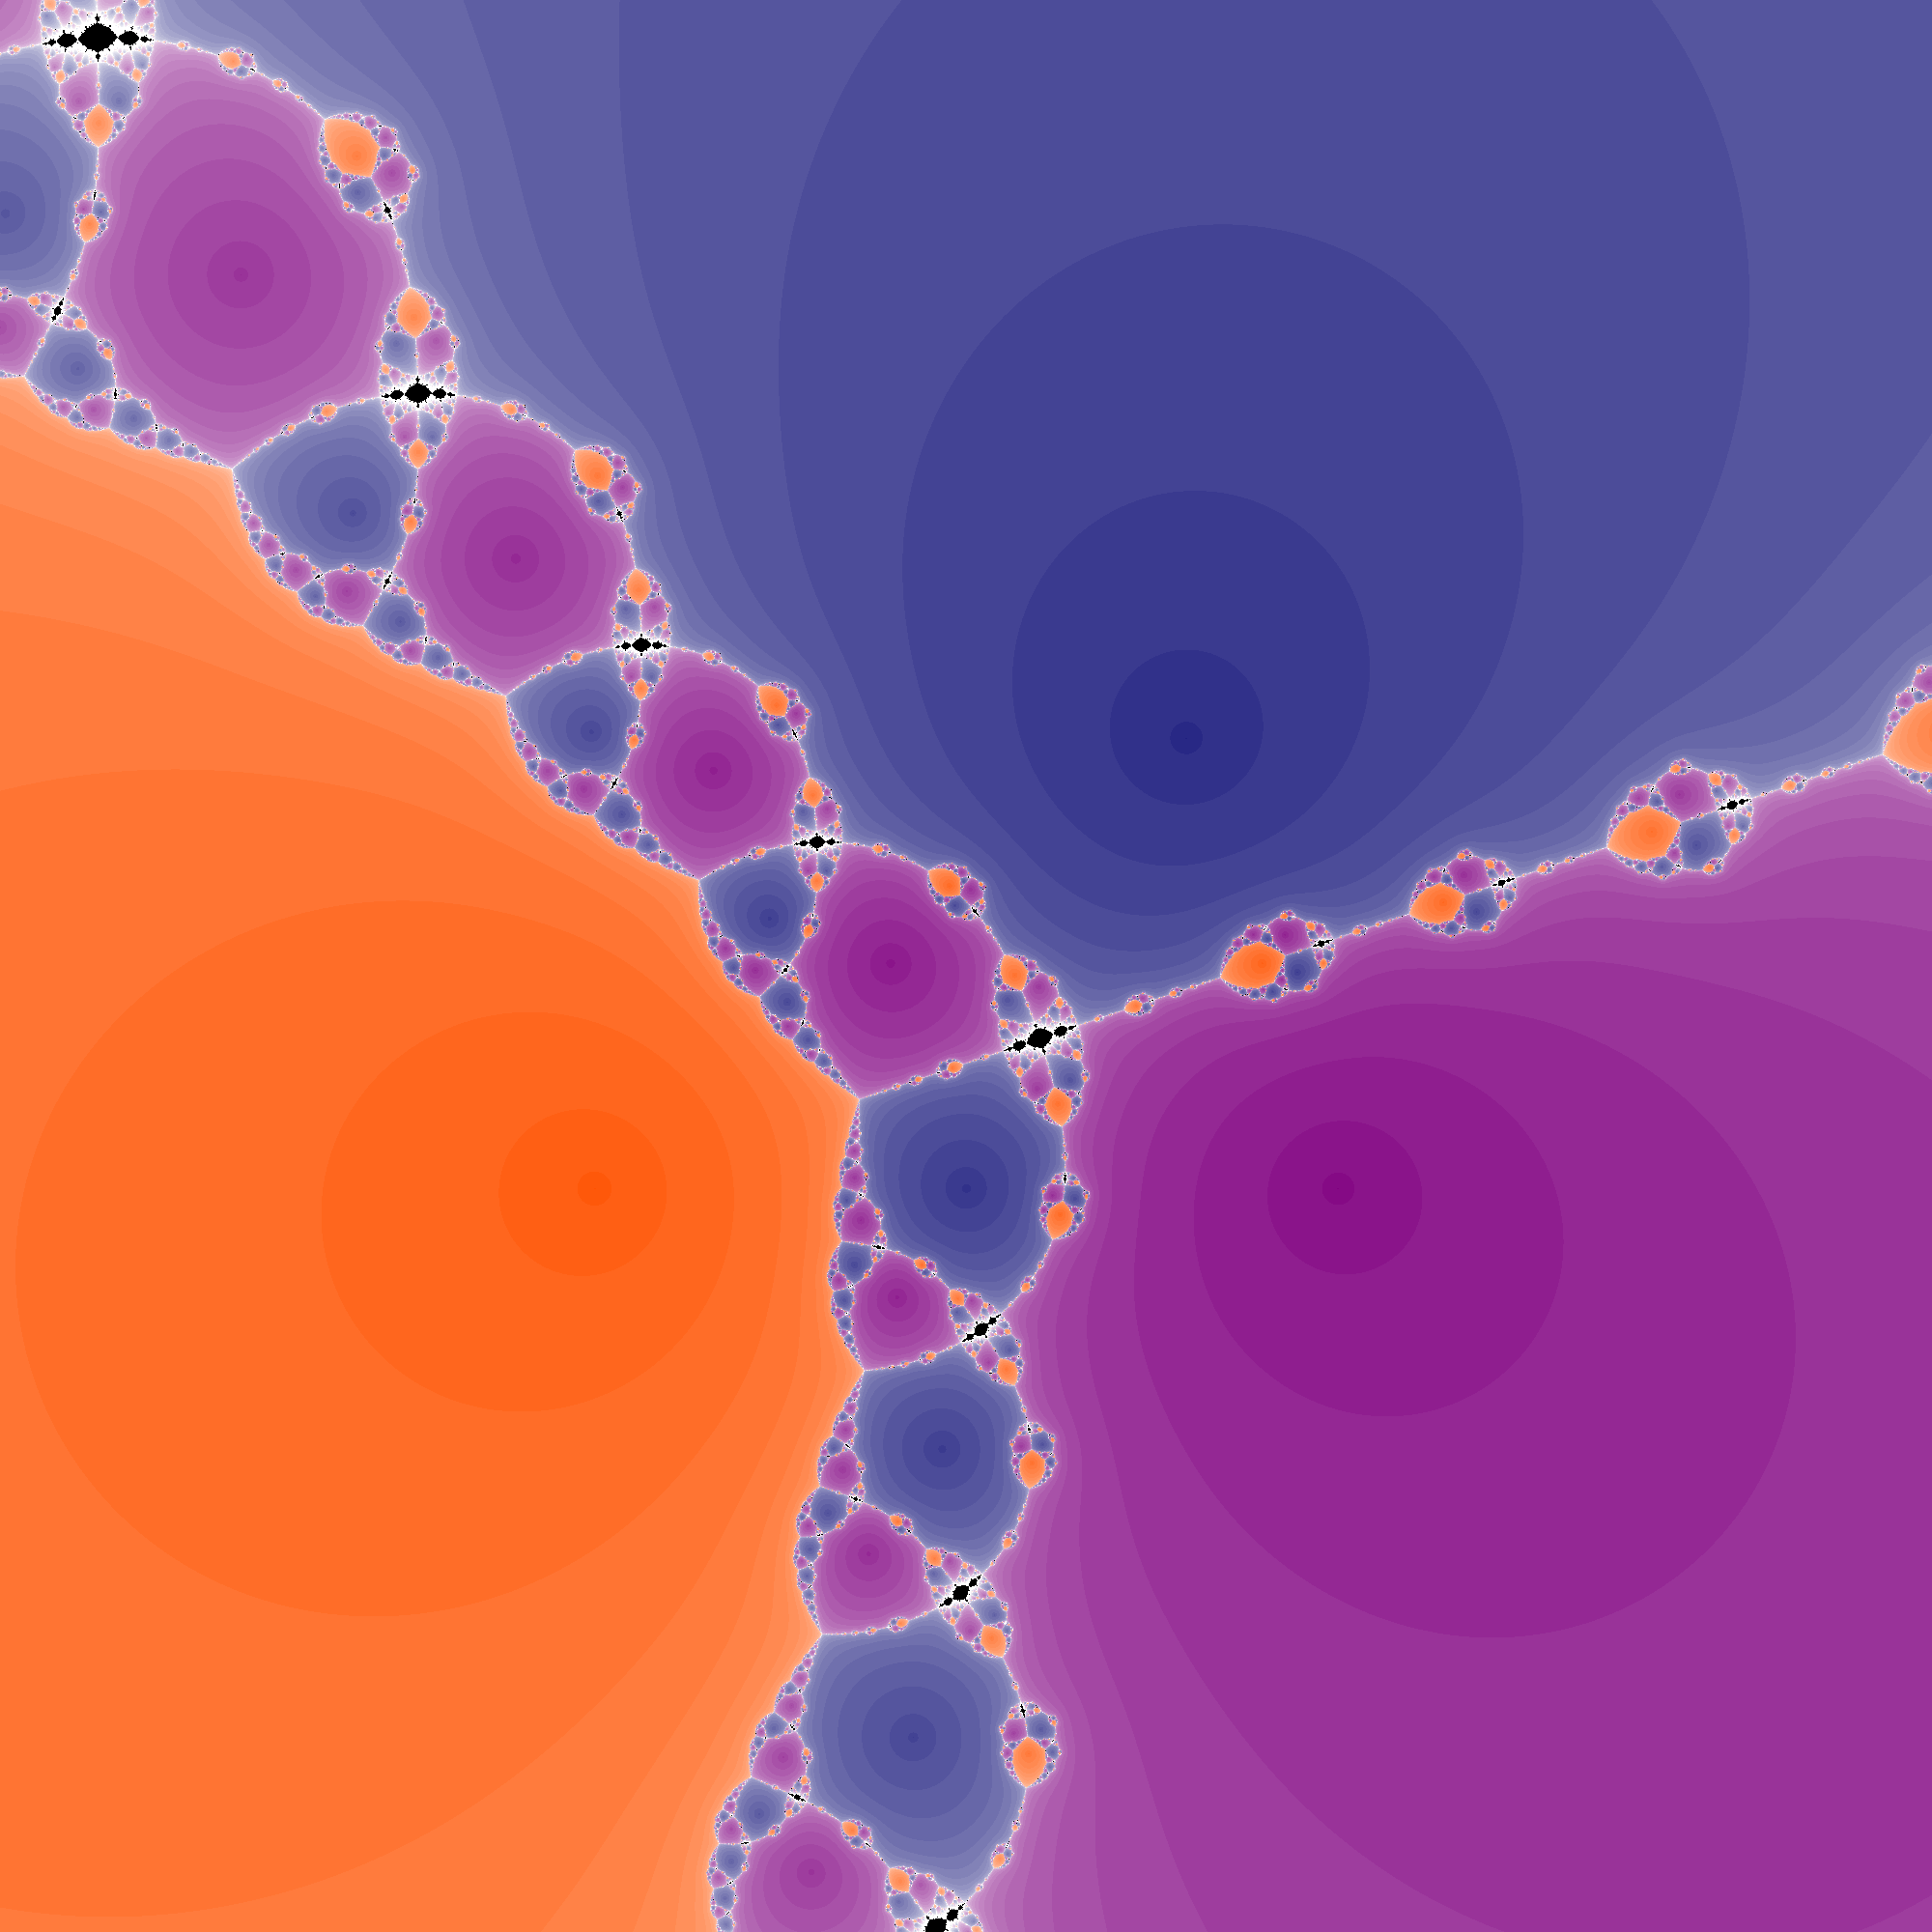
\includegraphics[width=\textwidth]{fig14a.png}
    \end{subfigure}
    \hfill
    \begin{subfigure}[b]{0.48\textwidth}
        \centering
        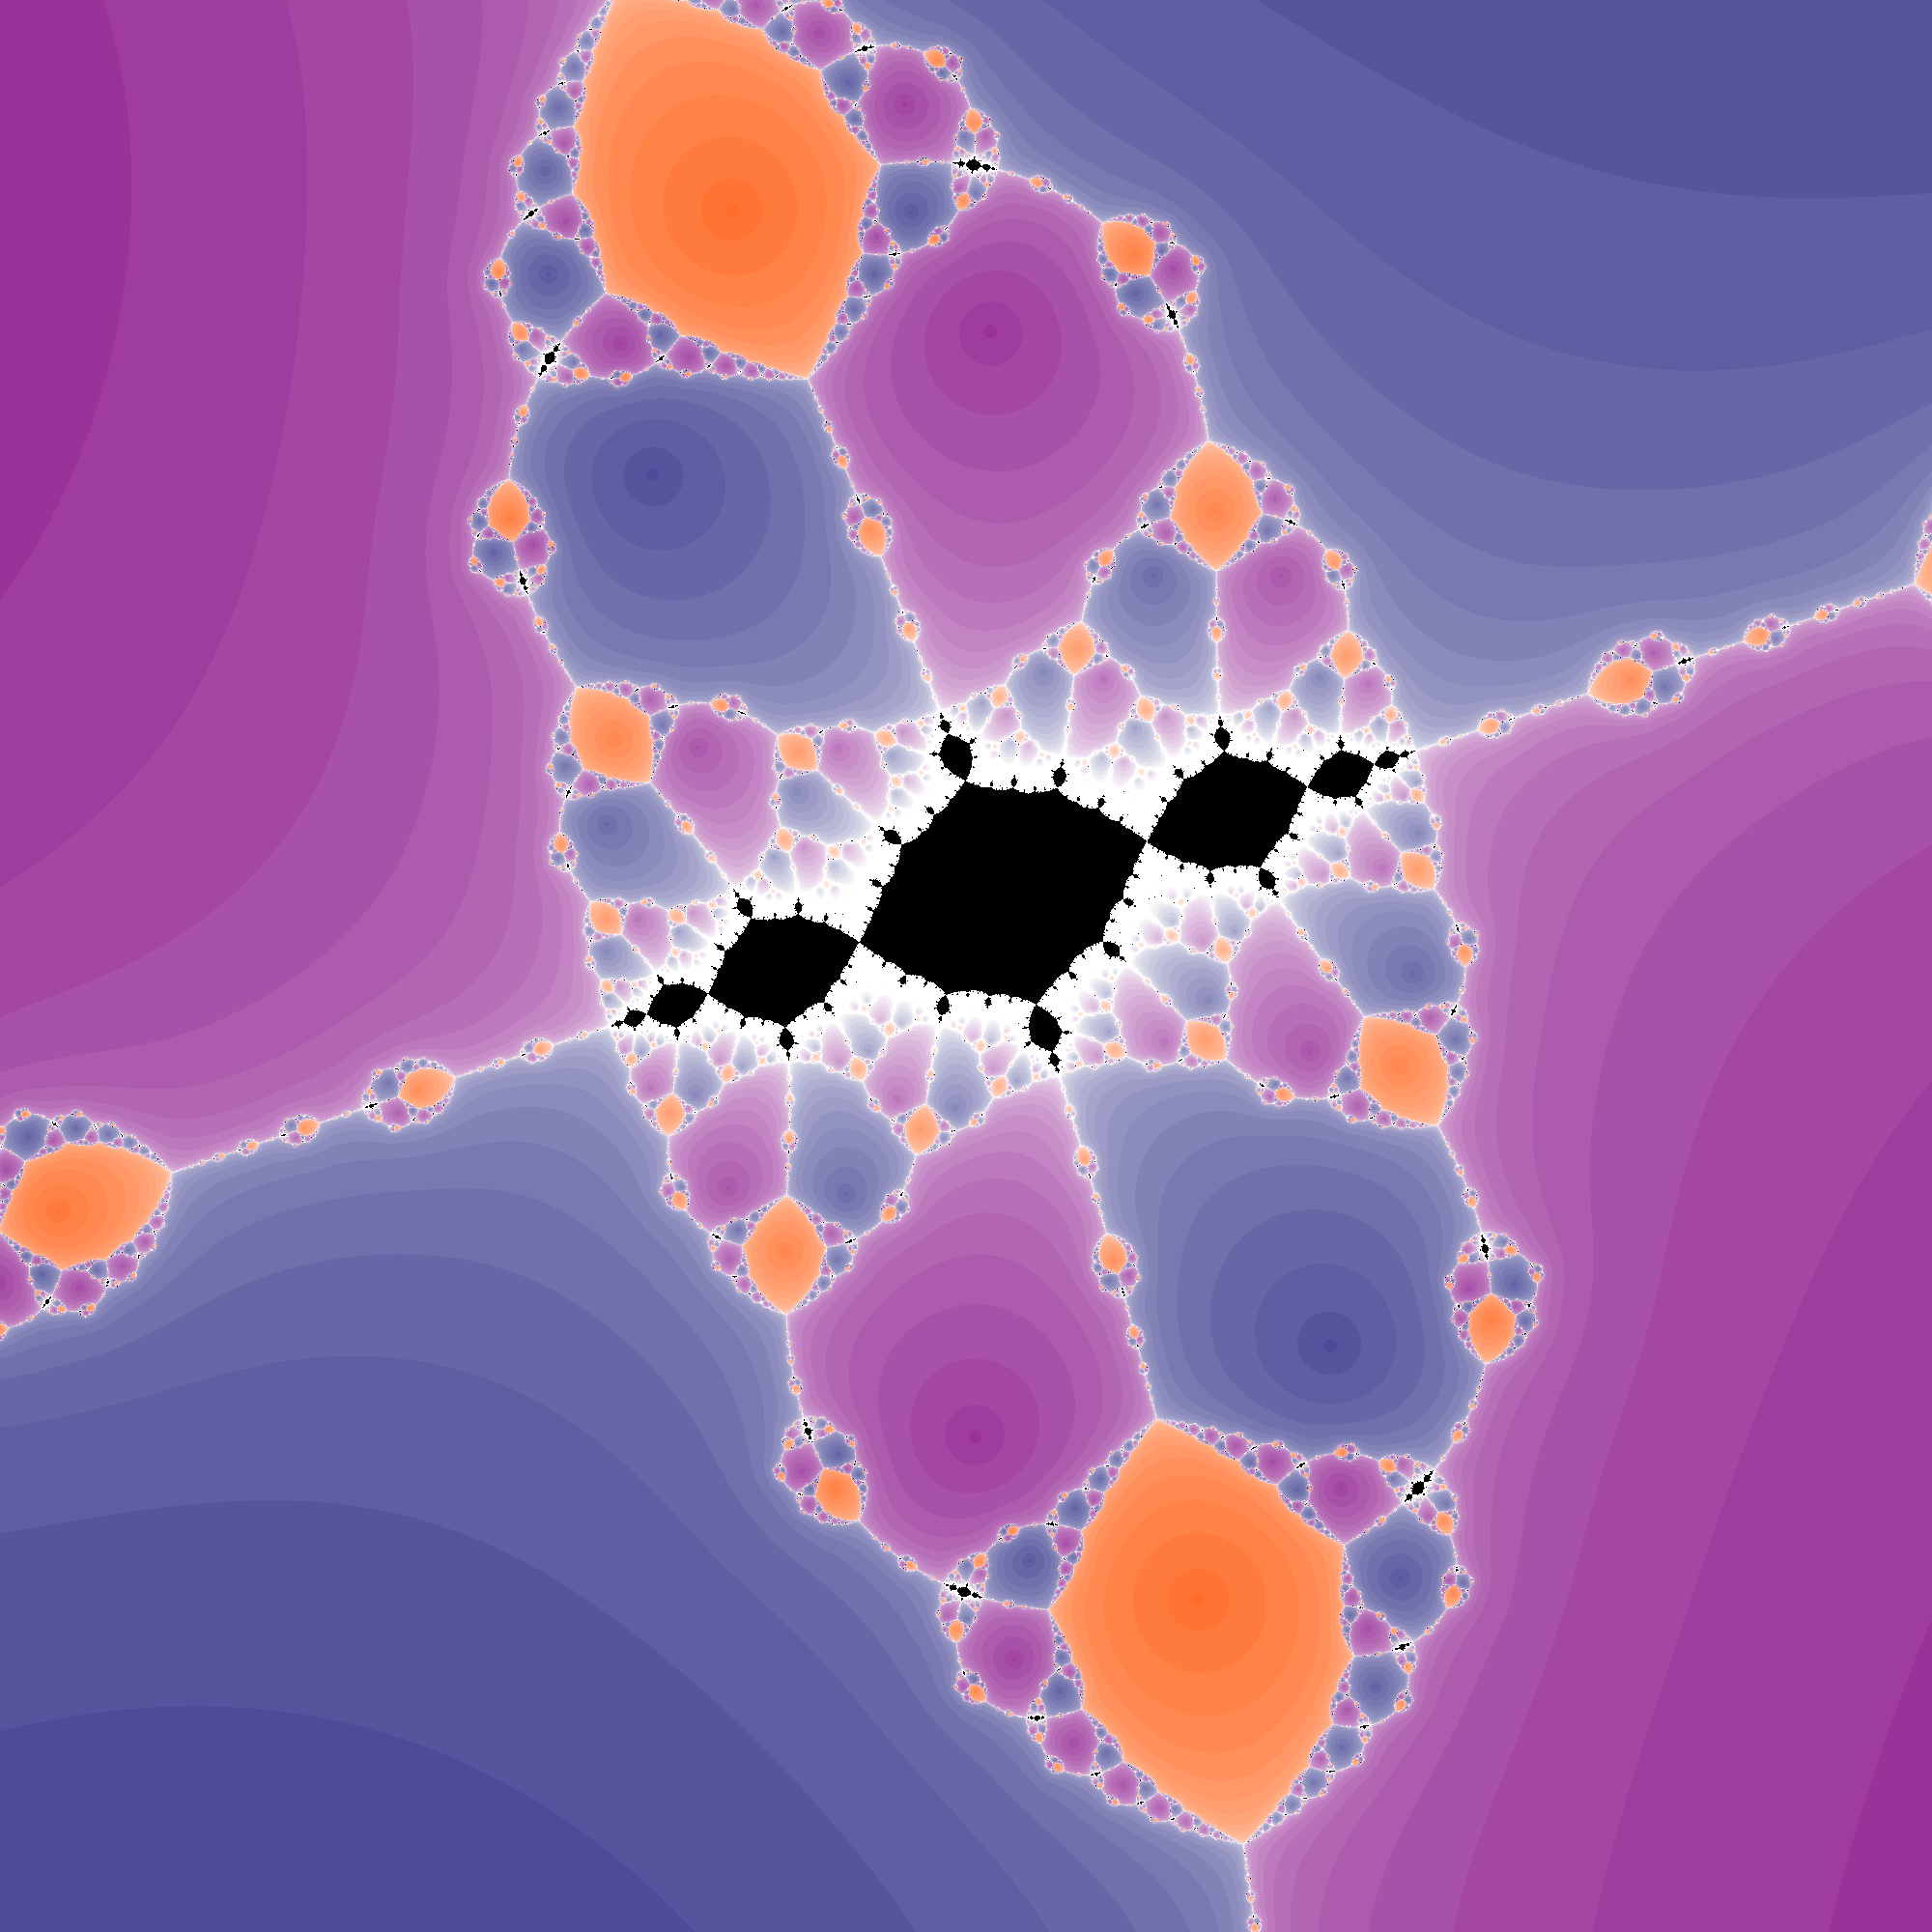
\includegraphics[width=\textwidth]{fig14b.png}
    \end{subfigure}
    \caption{\textbf{Left:} the phase plane of Newton's method of the
    polynomial $P(z)=z(z-1)(z-a)$ with $a$ chosen appropriately. \textbf{Right:} a
    zoom in which we see one of the sets of bad initial conditions. In this
    concrete case, it consists of the basin of attraction of a periodic orbit of
    period 2.}
    \label{fig:14}
\end{figure}

We can expect not to see the initial conditions of the Julia set in black, since
having measure zero, they will certainly not be on the computation grid. Even
so, we will see them almost white thanks to the gradation of colors, since the
closer an initial condition is to $\mathcal{J}$, the longer its orbit will take
to approach the corresponding root. In Figures~\ref{fig:3}, \ref{fig:6}, and
\ref{fig:14}, we can see that no black set is observed, which indicates to us
that probably the two polynomials chosen in those cases do not have bad initial
conditions for Newton's method, apart from those of the Julia set. But a
different case is seen with the polynomial of Figure~\ref{fig:14}, where the
existence of sets with positive measure that do not belong to any basin of
attraction is obvious. With any enlargement, these sets of bad initial
conditions become perfectly visible.

Once their existence is established, it is natural that we ask ourselves how
many of these sets we can find in a dynamic plane. The probable answer is that
there are infinitely many of them, since normally stable components have
infinitely many preimages. But it would be interesting to know how many
``different'' ones we can find. In the example of Figure~\ref{fig:14} we see an
infinity of black ``spots''. Taking some of them at random and with a few
calculations we could check that they all correspond to a basin of attraction of
a periodic orbit of period 2. In other words, it seems that all bad initial
conditions, apart from those in $\mathcal{J}$, have orbits that converge to the
same attracting periodic orbit. That is, it seems that they all belong to the
same basin of attraction. But how do we know this for sure?

\subsection{Entire Fatou components and singularities of the inverse}

We will say that $\mathcal{U}$ is a \textbf{grand Fatou component} if it is the
grand orbit of a connected component of the Fatou set. When we consider a grand
orbit, we have an open, totally invariant set, typically formed by infinitely
many connected components.

The problem of the previous section can be reformulated in general and in terms
of grand Fatou components. Given a specific function $F$, how do we know which
grand Fatou components are in its dynamic plane? How many different ones can
there be? To answer this question, we must talk about the singularities of
$F^{-1}$. For simplicity, we will assume, as we have done so far, that $F$ is a
rational function, as would be the case for Newton's method of a polynomial.

Any rational function $F(z)=\frac{Q_{1}(z)}{Q_{2}(z)}$ is a continuous and
analytic function at all points when we consider it as a function on the Riemann
sphere, i.e., on $\hat{\mathbb{C}}=\mathbb{C}\cup\{\infty\}$. In addition, $F$
is a local homeomorphism in a neighborhood of all its points, except in
neighborhoods of the zeros of the derivative $F^{\prime}$. This motivates the
following definition.

\begin{definition}
We say that $c$ is a \textbf{critical point} of $F$ if $F^{\prime}(c)=0$. Then,
$v=F(c)$ is called a \textbf{critical value} and is a singularity of $F^{-1}$,
in the sense that the branch of $F^{-1}$ that maps $v$ to $c$ is not
well-defined in any neighborhood of $v$ (inverse function theorem).
\end{definition}

Since $F$ is a quotient of polynomials, it only has a finite number of critical
points, $2d-2$ to be precise, where $d$ is the maximum degree between $Q_{1}$
and $Q_{2}$. These points play a crucial role in the dynamics of $F$, as shown
by the following theorem.

\begin{theorem}[\cite{7, 8}]
If $\mathcal{U}\subset\mathcal{F}(F)$ is a grand Fatou component, then
$\mathcal{U}$ has at least one associated critical point. More specifically:
\begin{itemize}
    \item Basins of attraction and parabolic basins contain at least one
    critical point.
    \item Siegel disks and Herman rings have the orbit of some critical point
    that accumulates on their boundary (in fact, two for the ring!).
\end{itemize}
\end{theorem}

We want to emphasize that this fact is very particular to analytic functions of
one variable. Nothing similar is true for differentiable dynamical systems, nor
for analytic ones looked at only on the real line, except in very special cases.

Observe that this provides us with great control over the stable sets. In some
way, we only need to iterate the critical points to locate all possible stable
components.

\section{Newton's method and its parameter plane}

Finally, we would like to apply again the general concepts we have seen to
Newton's method. For the previous theorem, it is important to see first what the
critical points of $N_{P}$ are and what their orbits are like.

If $P$ is a polynomial of degree $k>2$, the critical points of Newton's method
$N_{P}(z)=z-\frac{P(z)}{P^{\prime}(z)}$ are the solutions of
\begin{equation*}
    N_{P}^{\prime}(z)=\frac{P(z)P^{\prime\prime}(z)}{(P^{\prime}(z))^{2}}=0.
\end{equation*}

Therefore (assuming simple roots of $P$):
\begin{equation*}
    \{\text{Critical points of } N_{P}\} = \{\text{Zeros of } P\} \cup \{\text{Zeros of } P^{\prime\prime}\}.
\end{equation*}

The former are the roots of $P$ that we have called $\alpha_{1}, \dots,
\alpha_{k}$ and which are already the critical points associated with their
respective basins of attraction.

But the latter are the inflection points of $P$ (there are $k-2$ of them) and
these remain free to generate, or not, other Fatou components. In other words,
Newton's method $N_{P}$ can have at most $k-2$ grand Fatou components different
from the basins of attraction of the roots of $P$, one for each free critical
point.

Let us study in more detail the special case of polynomials of degree 3. For a
cubic polynomial, $N_{P}$ has four critical points: the three roots of $P$,
$\alpha_{1}, \alpha_{2}, \alpha_{3}$, and a free critical point, let us call it
$c$. As we have seen, the behavior of the orbit of the critical point,
$\mathcal{O}^{+}(c)$, gives us information about the possible grand Fatou
components that we can find in the dynamic plane, different from the basins of
attraction $\mathcal{A}(\alpha_{1}), \mathcal{A}(\alpha_{2}),
\mathcal{A}(\alpha_{3})$, the union of which we have called $\mathcal{A}$. For
example, in the case where the critical point $c$ is attracted by one of the
roots, it can no longer be generating any other stable component. This gives us
a sufficient condition, though not necessary, for a specific Newton's method to
work at almost every point of the plane (assuming that the Julia set has measure
zero):
\begin{equation*}
    \mathcal{O}^{+}(c)\rightarrow \alpha_{i} \text{ for some } i\in\{1,2,3\} \Rightarrow \mathcal{F}(N_{P})=\mathcal{A}
\end{equation*}
and, therefore, the only ``bad'' initial conditions are found in $\mathcal{J}$.
When this is not the case, there is the possibility (not the obligation) that
other grand Fatou components exist.

This condition can be checked by Newton's method for each polynomial in
particular. It is a fact, not difficult to verify, that every cubic polynomial
is conjugate by an affine map to another of the form
\begin{equation*}
    P_{a}(z)=z(z-1)(z-a).
\end{equation*}

It is, therefore, sufficient to study the family $P_{a}$ to know how the
Newton's methods of all polynomials of degree 3 behave. For this family, once
the value of $a$ is fixed, we would have to iterate the free critical point
$c_{a}=\frac{a+1}{3}$ (the zero of $P^{\prime\prime}$). We can show the result
in the complex plane, where each point of the plane represents a value of the
parameter $a$, and where we paint the point with different colors depending on
whether the orbit of $c_{a}$ is attracted by some of the roots (colors blue,
purple, or orange) or is not attracted by any (black).

\begin{figure}[htbp]
    \centering
    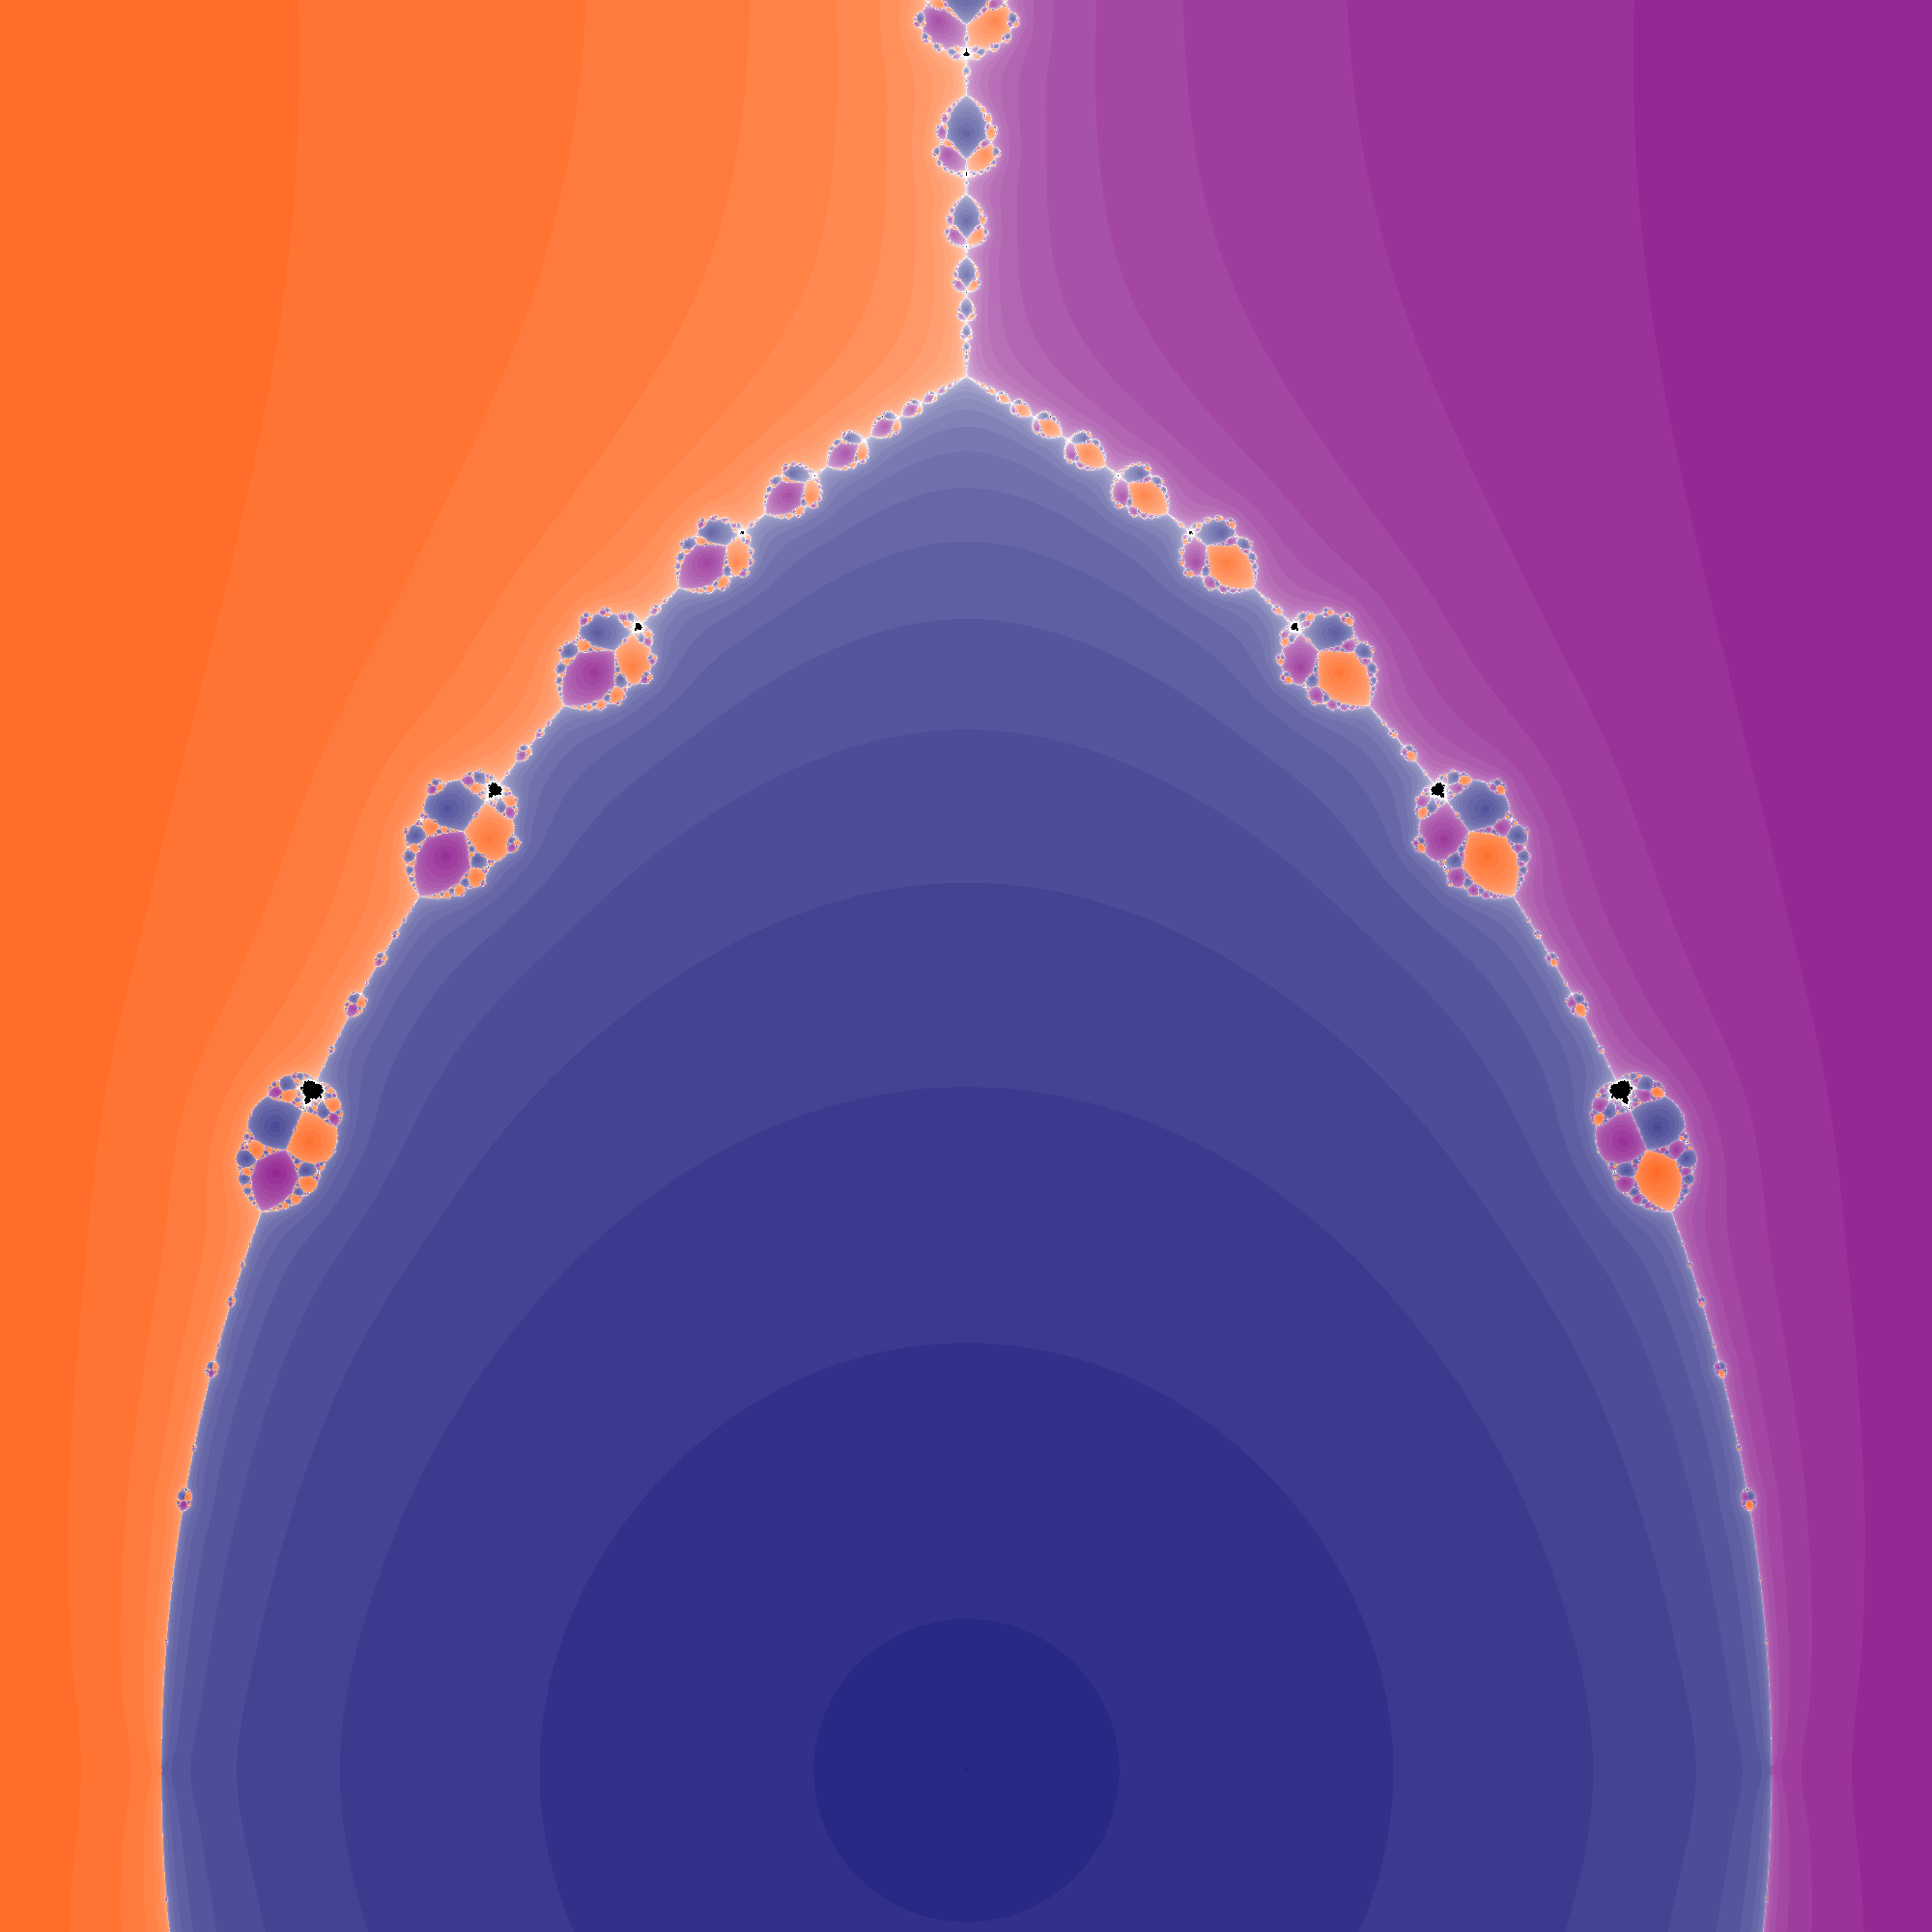
\includegraphics[width=0.6\textwidth]{fig15.png}
    \caption{Parameter plane of Newton's method for the family of cubic
    polynomials $P_{a}(z)=z(z-1)(z-a)$. Each point of the plane represents a value
    of $a$ and is colored if the orbit of the free critical point is attracted by
    some of the roots 0, 1, or $a$, and is black if it has any other behavior.}
    \label{fig:15}
\end{figure}

In this figure, we can then observe a multitude of black spots, apparently open
sets of parameter values, for which Newton's methods of the corresponding
polynomials possibly have sets of positive measure of bad initial conditions. In
Figure~\ref{fig:16} (left), a zoom is shown around one of these black spots,
where we see that the spot in question does not have just any shape. Quite the
contrary, the set we see is a (quasiconformal) copy of the celebrated Mandelbrot
set $M$, the bifurcation set of the quadratic family $Q_{c}(z)=z^{2}+c$, as
shown in Figure~\ref{fig:16} (right). This is the parameter plane of the
polynomials $Q_{c}$ (not of their Newton's methods!), and what we see is the
result of iterating their critical point $z=0$ for the different polynomials
$Q_{c}$, coloring the values of $c$ according to the behavior of this orbit.

\begin{figure}[htbp]
    \centering
    \begin{subfigure}[b]{0.48\textwidth}
        \centering
        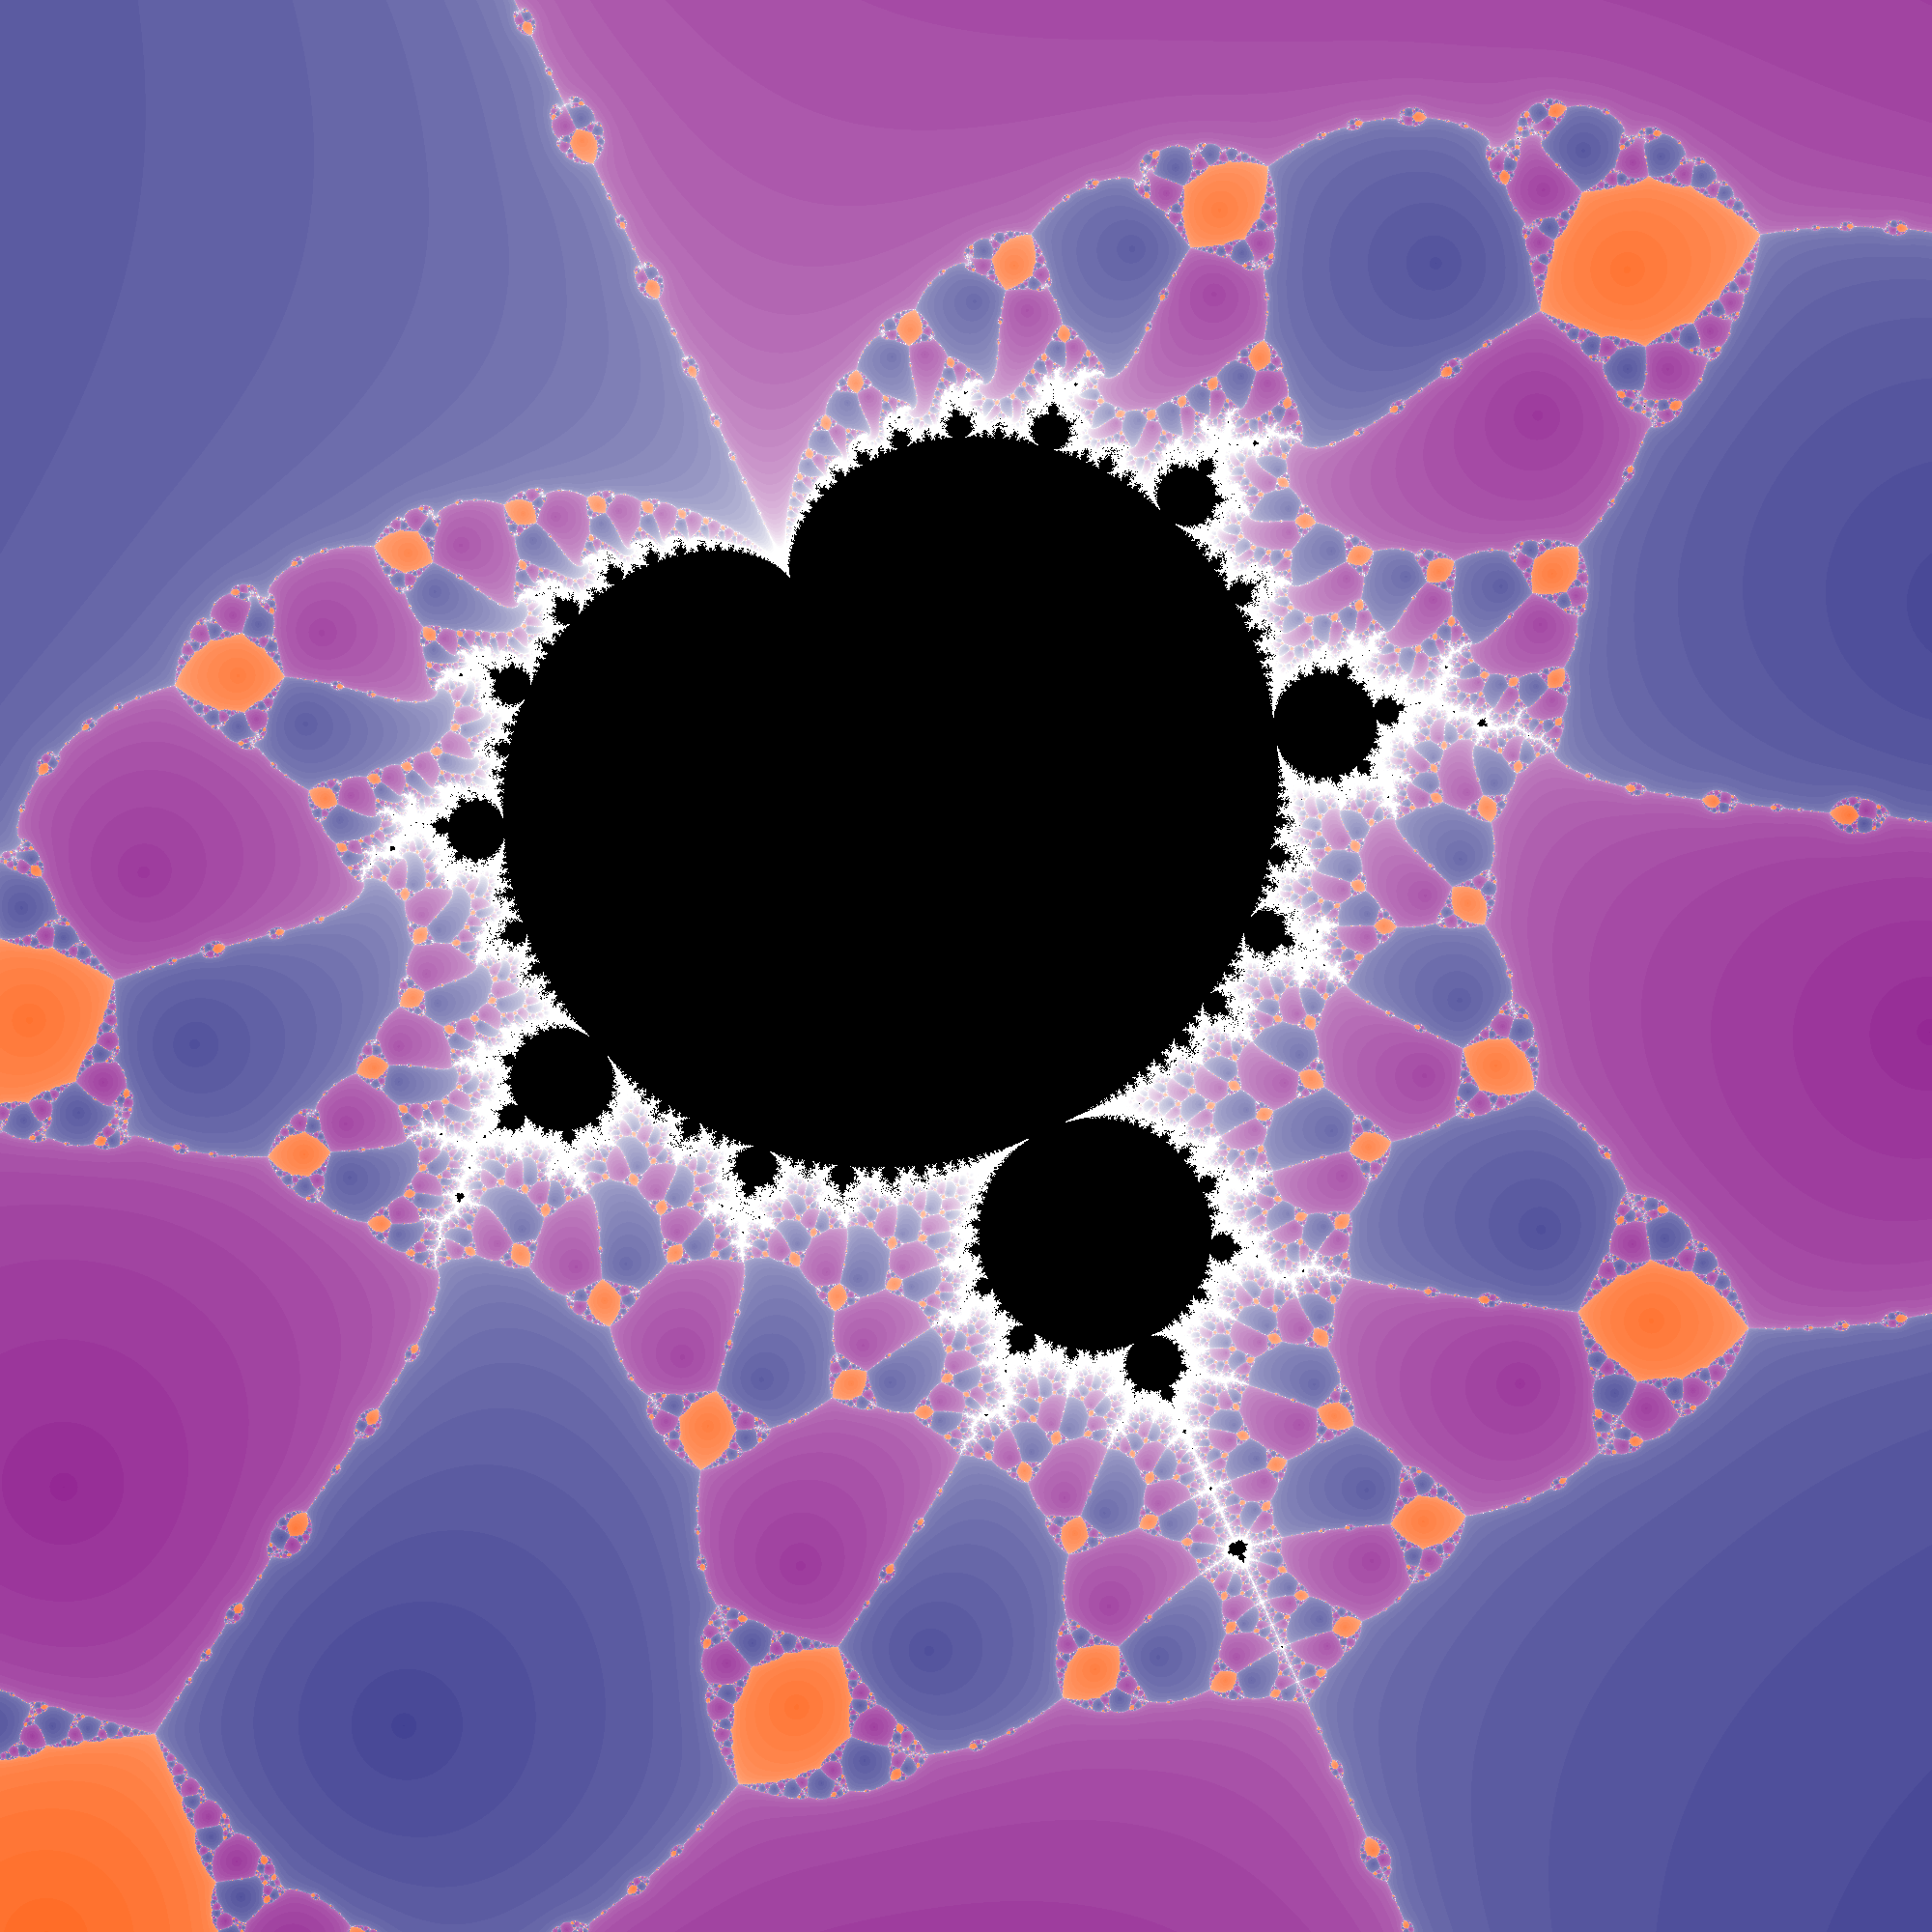
\includegraphics[width=\textwidth]{fig16a.png}
    \end{subfigure}
    \hfill
    \begin{subfigure}[b]{0.48\textwidth}
        \centering
        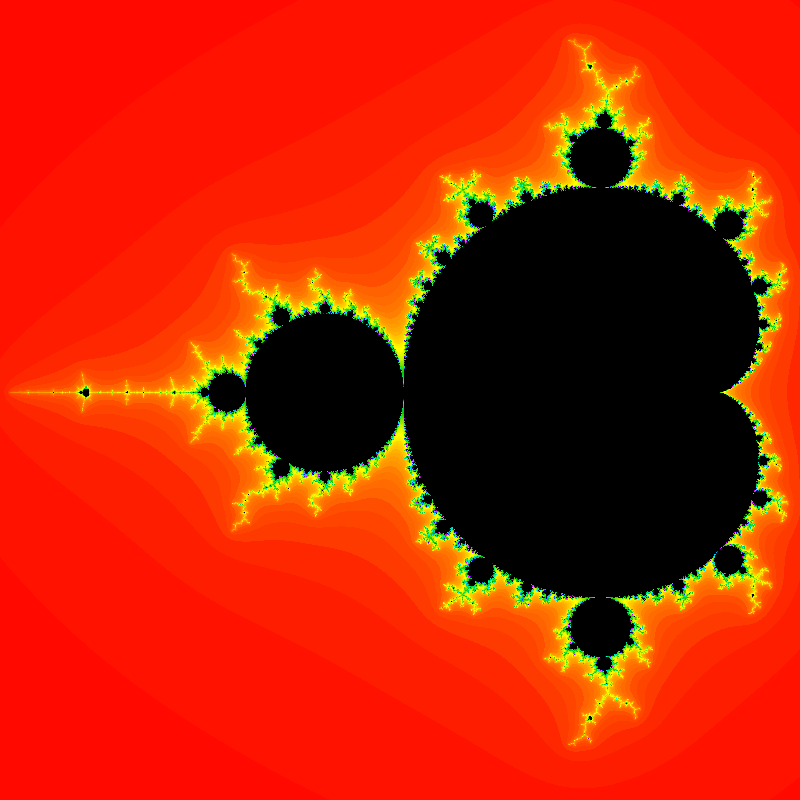
\includegraphics[width=\textwidth]{fig16b.png}
    \end{subfigure}
    \caption{\textbf{Left:} zoom around one of the small black spots of
    Figure~\ref{fig:15}. \textbf{Right:} the Mandelbrot set, in the parameter
    space of quadratic polynomials $Q_{c}(z)=z^{2}+c$ (not of their Newton's
    methods!). In other words, the result of iterating the critical point $z=0$
    for each of the polynomials $Q_{c}$.}
    \label{fig:16}
\end{figure}

The ``unexpected'' appearance of the Mandelbrot set in a parameter space foreign
to the family $Q_{c}$ is neither accidental nor strange. We know it is not
accidental, as it was explained in detail in 1985 by means of the theory of
polynomial-like mappings by Douady and Hubbard \cite{5}. This theory can be
summarized by saying that functions of all kinds, under certain conditions,
behave locally like polynomials. This is why we see polynomial Julia sets in
their dynamic planes (see Figure~\ref{fig:14} and compare it with
Figure~\ref{fig:8}), and Mandelbrot sets (or other analogue ones of higher
degree) in their parameter spaces. From this relationship, much information is
deduced about the dynamics for the parameters that live inside these copies of
$M$. For example, we will highlight one fact: for all parameters in the interior
of a copy of $M$, the corresponding dynamic planes have an attracting periodic
orbit and, therefore, a basin of attraction, or else the Julia sets have
positive measure. We deduce, therefore, that we have open sets of parameters
(all the interiors of the copies of $M$) for which Newton's methods fail on sets
of positive measure.

We will end this lecture by remarking that finding copies of the Mandelbrot set
in various parameter spaces is not at all strange, since the conditions required
for this to happen are relatively common and, indeed, occur in a multitude of
families of all kinds; not only rational like those that have occupied us, but
also transcendental. Because of this fact, we say that the Mandelbrot set is a
universal set. And this is also why the Mandelbrot set has been and continues to
be an object of great interest to a multitude of mathematicians, especially also
because it is an inexhaustible source of open problems, many of which have
resisted being solved to this very day.

\begin{thebibliography}{99}

\bibitem{1} BRJUNO, A. D. ``Analytic form of differential equations.''
\emph{Trans. Mosc. Math. Soc.}, 25 (1971).

\bibitem{2} CAYLEY, A. ``Applications of the Newton-Fourier Method to an
imaginary root of an equation.'' \emph{Quat. J. of Pure and App. Math.}, 16
(1879), 179--185.

\bibitem{3} CAYLEY, A. ``The Newton-Fourier Method imaginary problem.''
\emph{Am. J. of Math.}, 2 (1879), 97.

\bibitem{4} CAYLEY, A. ``On the Newton-Fourier imaginary problem.'' \emph{Proc.
Camb. Phil. Soc.}, 3 (1880), 231--232.

\bibitem{5} DOUADY, A.; HUBBARD, J. ``On the dynamics of polynomial-like
mappings.'' \emph{Ann. Scient. Ec. Norm. Sup.}, 18 (1985), 287--343.

\bibitem{6} FATOU, P. ``Sur les équations fonctionelles.'' \emph{Bull. Soc. mat.
Fr.}, 47 (1919), 161--271; 48 (1920), 33--94, 208--314.

\bibitem{7} FATOU, P. ``Sur les substitutions rationnelles.'' \emph{Comp. Rend.
heb. S. Acad. Sci.}, 164 (1917), 806--808; 165 (1917), 992--995.

\bibitem{8} JULIA, G. ``Mémoire sur l'iteration des fonctions rationnelles.''
\emph{J. Math. Pures Appl.}, 8 (1918), 47--245.

\bibitem{9} SCHRÖDER, E. ``Ueber unendlich viele Algoritheoremen zur Auflösung der
Gleichungen.'' \emph{Mathematische Annalen}, 2 (1870), 317--365.

\bibitem{10} SCHRÖDER, E. ``Ueber iterirte Functionen.'' \emph{Mathematische
Annalen}, 3 (1871), 296--322.

\bibitem{11} SULLIVAN, D. ``Quasiconformal homeomorphisms and dynamics.''
\emph{Annals of Math.}, 122 (1985), 401--418.

\end{thebibliography}

\end{document}